\documentclass[draft,12pt]{report} %use draft mode for rendering tests for formatting but not for the final verson e.g. \documentclass[12pt]

\usepackage{graphicx} 
\usepackage{setspace}
\usepackage{float} %needed to force figures in certain place
\usepackage{url}

% %avoid widows and orphans - really important for references
% \widowpenalty10000
% \clubpenalty10000
\usepackage[all]{nowidow}




%needed for continuous footnote numbering (requires d/l of chngcntr.sty)
\usepackage{chngcntr}
\counterwithout{footnote}{chapter}

%probably not necessary but may affect output quality if changed
\pdfcompresslevel=1

%set tab to be 0.5 in
\setlength{\parindent}{.5in}

\usepackage{natbib}
\usepackage{chapterbib}


%this makes references be a section style rather than chapter stile
%still need to manually add it to TOC in the paper tex file and change the name to REFERNCES
\makeatletter
\renewcommand\bibsection%
{
  \section*{\refname
    \@mkboth{\MakeUppercase{\refname}}{\MakeUppercase{\refname}}}
}
\makeatother
%this removes the ``references'' defined by natbib, and lets you use section names instead,
%which automatically adds it to TOC. Needs the above code to treat refs section as section and not chapter
\renewcommand{\bibsection}{}




%\usepackage{url}
\doublespacing
% \numberwithin{equation}{section}
\usepackage[top=1in, bottom=1in, left=1in, right=1in]{geometry}
\usepackage{amsmath}
\setcounter{secnumdepth}{5} %this allows use of subsubsections
\setcounter{tocdepth}{5}
\usepackage{graphicx}
%the next three lines are more friendly to foreign (icelandic) fonts
\usepackage[T1]{fontenc}
\usepackage{lmodern} %this is needed with T1
\usepackage[utf8]{inputenc}
\usepackage{listings}

%\renewcommand{\chaptername}{}
%\renewcommand{\thechapter}{}

%perform USF style heading formats
%\newcommand{\cchapter}[1]{\chapter[#1]{\centering #1}}
\usepackage{titlesec}

%needed to not center abstact vertically on center of page and bring it to top instead
\usepackage{etoolbox}

%TOC stuff
\usepackage{alltt}
%TOC INDENTATION
\usepackage[titles]{tocloft}




%control chapter heading PROBABLY NOT NEEEDD
% \titleformat{\chapter}[display]
% 	{\normalfont\Luge\bfseries\centering}{\chaptertitlename\ \thechapter}{20pt}{\Huge}

%next three blocks control heading indents	
\titlespacing{\chapter}{0em}{.68in}{2em}
\titleformat{\chapter}
  {\normalfont\bfseries\centering}{\thechapter}{1em}{}

\titlespacing{\section}{0em}{1em}{0em}
\titleformat{\section}
  {\normalfont\bfseries\raggedright}{\thesection}{1em}{}

\titlespacing{\subsection}{.5in}{1em}{0em}
\titleformat{\subsection}
  {\normalfont\bfseries}{\thesubsection }{1em}{}
  

%disable section and subsection numbering
%\setcounter{secnumdepth}{0} 

%suppress chapter numbering
%\renewcommand{\thechapter}{}


%format the table of contents
\makeatletter
\def\tableofcontents{%
 \newpage
\vspace*{.82in}
 \centerline{\bf Table of Contents}
 \vspace*{2em}
 \@mkboth{CONTENTS}{CONTENTS}
 \@starttoc{toc}
}
\makeatother

%format the list of figures (if you have list of tables, this needs to be repated)
\makeatletter
\def\listoffigures{%
 \newpage
\vspace*{.80in}
 \centerline{\bf List of Figures}
 \vspace*{2em}
 \@mkboth{CONTENTS}{CONTENTS}
 \@starttoc{lof}
}
\makeatother




%get rid of leader dots in TOC and LOF
\renewcommand{\cftdot}{}


%this part of the code ensures that there is a period after the number, e.g. 1. CHAPTERNAME
\makeatletter
\renewcommand{\@makechapterhead}[1]{%
{ \vspace*{.5in} }
{\setlength{\parindent}{0pt} \center \normalfont
\bfseries\thechapter.\ #1
\par\nobreak\vspace*{\baselineskip}}}
\makeatother


%figure stuff - leave as is (may be important if figures are inside the text rather htan at the end of the chapters)
\widowpenalty=10000
\clubpenalty=10000


%this controls the TOC indentation
\renewcommand{\cftsecindent}{.5in}
%\renewcommand{\cftsecnumwidth}{1.9 em}
\renewcommand{\cftsubsecindent}{1in}
%\renewcommand{\cftsubsecnumwidth}{2.8 em}	
\renewcommand{\cftfigfont}{Figure }
%these should change the table of contents main headings to not be bold
\renewcommand\cftchapfont{\mdseries}
\renewcommand\cftchappagefont{\mdseries}


%define page nums to be .25" below text
\setlength{\footskip}{0.25in}

%this should set indent level for Figure X....(0 inches so that its at left margin)
\setlength{\cftfigindent}{0in}
%note that the Figure X and the rest of the text are tied, so the above value should be 0


%this controls vertical spacing, NECESSARY FOR DOUBLE SPACING BETWEEN TITLES
\setlength{\cftbeforefigskip}{1em}
%this controls distance between figure X: ____ NAME
% \setlength{\cftfignumwidth}{.5in}

%this is needed to keep proper indentation in two-line figure label text
%ALL OF THESE ARE NECESSARY
\renewcommand{\cftfigfont}{}
\renewcommand{\cftfigpresnum}{Figure }             	
\renewcommand{\cftfigaftersnum}{}  
\renewcommand{\cftfigpagefont}{}                      
\renewcommand{\cftfignumwidth}{1in}



%this may add colon somewhere in the TOC/LOF ???
% \renewcommand{\cftXaftersnum}{:}
% 


%this will redefine the width of the pagenumbering on the TOC/LOF (3 font units (e.g. for pages containing three characters like 113)
\makeatletter\renewcommand{\@pnumwidth}{3em}\makeatother

%this lets the chapter names and figure captions end at 0.5 in from the right per usf rules
\makeatletter\renewcommand{\@tocrmarg}{0.5in}\makeatother

%remove extra space in List of Figures between header and the figure list
\addtocontents{lof}{\protect\renewcommand*\protect\addvspace[1]{}}
%MUST DO SAME FOR TOC, NOT YET DONE????????

%control spacing inside LOF
%???????
% \renewcommand{\cftfigafterpnum}{1.25in}
%
%\makeatletter
%\def\@makeschapterhead#1{%
%  \vspace*{.6in}% space before the title
%  {\center
%    \normalfont
% \bfseries  #1\par\nobreak
%    \vskip 12\p@ % space after the title
%  }}
%\makeatother

%this is an OVERFULL eliminator - if black rectangle appears in text, this gets rid of it DO NOT REMOVE THIS 
\setlength{\emergencystretch}{2em}

%needed to not center abstact vertically on center of page and bring it to top instead
% \usepackage{etoolbox}
% \patchcmd{\abstract}{\null\vfil}{}{}{}


\begin{document}

%TITLE PAGE FILE GOES HERE
\begin{titlepage}
\begin{center}
\singlespacing
% { \vspace*{\baselineskip} }
{ \vspace*{\baselineskip} }
{ \vspace*{\baselineskip} }
{ \vspace*{\baselineskip} }
{ \vspace*{\baselineskip} }
Modeling the Construction and Evolution of Distributed Volcanic Fields on Earth and Mars\\
{ \vspace*{\baselineskip} }
{ \vspace*{\baselineskip} }
{ \vspace*{\baselineskip} }
by\\
{ \vspace*{\baselineskip} }
{ \vspace*{\baselineskip} }
{ \vspace*{\baselineskip} }
Jacob A. Richardson\\
{ \vspace*{\baselineskip} }
{ \vspace*{\baselineskip} }
{ \vspace*{\baselineskip} }
{ \vspace*{\baselineskip} }
A dissertation submitted in partial fulfillment\\
of the requirements for the degree of\\
Doctor of Philosophy\\
School of Geosciences\\
College of Arts and Sciences\\
University of South Florida\\
{ \vspace*{\baselineskip} }
{ \vspace*{\baselineskip} }
{ \vspace*{\baselineskip} }
Major Professor: Charles B. Connor, Ph.D.\\
Jacob E. Bleacher, Ph.D.\\
Rocco Malservisi, Ph.D.\\
Matt A. Pasek, Ph.D.\\
Timothy H. Dixon, Ph.D.\\
{ \vspace*{\baselineskip} }
{ \vspace*{\baselineskip} }
Date of Approval:\\
Month day, Year\\
{ \vspace*{\baselineskip} }
{ \vspace*{\baselineskip} }
{ \vspace*{\baselineskip} }
Keywords: Volcanology, Planetology, Geomorphology, Remote Sensing, Statistics\\
{ \vspace*{\baselineskip} }
%the hspace is needed to put space beween the C and the year, which is not done by default
Copyright \copyright\hspace{1mm}2016, Jacob A. Richardson\\
\end{center}
\end{titlepage}



\pagenumbering{roman}
\begin{singlespace}
%\vspace*{1in}

\tableofcontents

\end{singlespace}


%not sure what this does
\renewcommand{\cftsecleader}{\cftdotfill{\cftdotsep}}



%LOF needs to have singlespacing between lines continued onto a second line. The extra spacing between each figure is forced elsewhere in the preamble.
\begin{singlespace}
% \cleardoublepage
% \addcontentsline{toc}{chapter}{List of Tables}
% \listoftables
\cleardoublepage % Start a new page for the list of figures. Make it right handed for two-sided documents.
\addcontentsline{toc}{chapter}{List of Figures} % add to table of contents.
\listoffigures % generate the list of figures
\end{singlespace}

% \renewcommand{\abstitleskip}{\vspace{-\baselineskip}}
%needed to not center abstact vertically on center of page and bring it to top instead
\patchcmd{\abstract}{\null\vfil}{\vspace*{37pt}}{}{}
\begin{abstract}
\thispagestyle{plain}
Terrestrial Radar Interferometry (TRI) is a relatively new ground-based technique that combines the precision and spatial resolution of satellite interferometry with the temporal resolution of GPS. Although TRI has been applied to a variety of fields including bridge and landslide monitoring, it is ideal for studies of the highly-dynamic terminal zones of marine-terminating glaciers, some of which are known to have variable velocities related to calving and/or ocean-forced melting. My TRI instrument is the Gamma Portable Radar Interferometer, which operates at 17.2 GHz (1.74 cm wavelength), has two receiving antennas for DEM (digital elevation model) generation, and images the scenes at minute-scale sampling rates.  Most of this TRI work has focused on two glaciers: Breiðamerkurjökull in Iceland and Helheim in Greenland. Monitoring the displacement of stationary points suggests velocity measurement uncertainties related to the instrument and atmosphere of less than 0.05 m/d. I show that the rapid sampling rate of the TRI can be used to observe velocity variations at the glacier terminus and assess the impact and spatial distribution of tidal forcing. Additionally, iceberg tracking in the amplitude imagery may provide insight about ocean currents near the terminus. 
\setcounter{page}{6} %NEEED TO MANUALLY SET PAGE HERE
%force abstract in the TOC
% \clearpage
\addcontentsline{toc}{chapter}{Abstract}
\end{abstract}


\pagenumbering{arabic}


%use the intro paragraph here, must define chapter and label in the other tex file
%need to remove all of the journal-specific formatting stuff from the tex files in the separate chapter files
\chapter[Introduction]{Introduction}

Distributed volcanism is a style of volcanic activity that forms clusters of volcanic edifices instead of building one large edifice in successive eruptions through a central vent \citep{valentine2000basaltic}. Each edifice in a volcanic field, often a scoria cone, lava dome, or maar diatreme, is most often created from the arrival of a single magmatic dike to the surface during a single eruptive phase that lasts from weeks to decades in length. The common term ``monogenetic volcano,'' used to describe scoria cones, small shield volcanoes, and maar volcanoes, comes from this concept of single eruptions forming small volcanoes \citep{greeley1977basaltic}, though individual scoria cones sometimes exhibit recurring volcanic activity in spite of this term \citep{hill1998cerro}. Distributed-style volcano clusters, forming from dikes ascending through lithosphere from a magma source hundreds to many thousands of square kilometers in extent, are reflections of both their source region and the lithosphere \citep{settle1979structure}.

People have lived within volcanic fields since pre-historic times and their livelihoods have been affected when eruptions occur, usually with little to no warning \citep{elson2007living}. Recently, spacecraft have been sent to other planets, revealing the existence of distributed-style volcanism, much like Earth's, on Mars \citep{carr1977some} and Venus \citep{head1992venus}. On these neighboring planets, tens to tens of thousands of distributed volcanic vents form patchworks of shield volcanoes \citep{richardson2013volcanic,miller2012shield}. 

This dissertation assembles five projects that explore different aspects of distributed volcanic fields. The first project focuses on the role of the magma plumbing system on evolution of volcanic fields. This project uses lidar datasets to model magmatic sills in the San Rafael, Utah and has been published as \citet{richardson2015sills}. Second, a lava flow simulator is validated and used to model a recent lava flow. This simulator has simulated the 2012-3 Tolbachik lava flow in Kamchatka, Russia, using flow characteristics derived from TanDEM-X InSAR data in \citet{kubanek2015lava}. Third, two chapters focus on volcano clusters on Mars, characterizing the long-term evolution of two fields. The first of these studies the Syria Planum region and has been published as \citet{richardson2013volcanic}. The second focuses on Arsia Mons and has been presented as \citet{richardson2015recurrence}. The final chapter models and compares the spatial density of volcanic vents in clusters on Earth, Mars, and Venus. This project has been presented as \citet{richardson2012comparison}. Chapters are roughly ordered in ascending distance from the Earth's center. 

\section{Role of sills in the development of volcanic fields}
In Chapter \ref{ch_sills}, terrestrial and airborne lidar data are used to map volcanic features in the San Rafael Swell (Utah, USA). These features make up the San Rafael Volcanic Field, a Pliocene-aged volcanic field that has been eroded away to a depth of $<$1~km exposing the igneous intrusion network. Analysis of the combined lidar datasets enables the modeling of the geometries of seven magmatic sills. The total volume of these sills is $>$0.4~km$^3$, with each sill containing 10$^{-4}$-10$^{-1}$ km$^3$ of igneous rock. Mapped sill volumes account for $>$92\% of intrusive material within the 50~km$^2$ study area, with the rest of the material being stored in dikes and volcano conduits.

Sills in the San Rafael likely played a significant role in modifying eruption dynamics during activity in San Rafael. At least one sill has been identified to have formed cotemporally with an eruption. Depending on the size of the conduit to the surface and the adjacent co-magmatic sill, gas would have been entrained in either the conduit or the sill, modulating explosivity of the eruption.

\section{Validating Lava Flow Simulators using a Validation Hierarchy and Bayesian Analysis}
In Chapter \ref{ch_molasses}, a cellular automata \citep{wolfram1984cellular} lava flow simulator is developed following the algorithm of \citet{connor2012probabilistic}. The simulator, named MOLASSES, has been developed in C with a modular framework, which enables users to quickly change relatively few lines of code to modify the flow behavior. While there are multiple ways to modify simulated flow behavior to model lava flows, each modified algorithm needs to be validated before it can be relied upon in the field. 

A validation strategy has been designed with the objective of comparing CA flow codes with bingham fluids and real life lava flows. To fulfill this objective, four validation levels have been devised, into which different tests can be applied to evaluate lava spreading algorithms against increasingly complex tests. These levels are 1) verification of the code by testing for conservation of mass; 2) testing for flow self-similarity given inconsequential variations in input parameters; 3) testing for replication of Bingham flow morphology on simple surfaces; and 4) testing for replication of real lava flow morphologies on pre-eruption elevation models. 

Model output uncertainty is then evaluated using two Bayesian posterior statistics, the Positive Predictive Value and the Negative Predictive Value. The 2012-3 Tolbachik lava flows are used as a test case. These metrics can provide insight into improving model performance and decision making in volcanic crises.

\section{The Volcanic History of Syria Planum, Mars}
In Chapter \ref{ch_syria}, a field of distributed shield volcanoes in the Syria Planum region of Mars is mapped to determine abundance, distribution, and alignments of vents. Nearest neighbor and two--point azimuth analyses are conducted, using mapped volcanic vent locations, to assess the spacing and orientations between vents across the study area. Two vent fields are identified as unique volcanic units along with the previously identified Syria Mons volcano. Superposition relationships and crater counts indicate that these three volcanic episodes span $\sim$900 Ma, beginning in the early Hesperian Period and ending in the Early Amazonian Period. No clear hiatus in eruptive activity is identified between these events, as crater age-dating error bars of each unit abut the modeled ages of other units. However, activity migrates from eruptions at Syria Mons, to regionally distributed eruptions that form the bulk of the Syria Planum plains, to dispersed eruptions in Syria's northwest. 

Nearest neighbor analyses suggest a non--random distribution among the entire population of Syria Planum, which is interpreted to result from the interaction of independent magma bodies ascending through the crust during different stress regimes throughout the region's eruptive history. Two--point azimuth results identify three orientations of enhanced alignments, which match well with radial extensions of three major tectonic centers to the south, east, and northwest of the study area. 

As such, Syria Planum volcanism evolved from a central vent volcano to dispersed shield field development over several hundred million years, during which the independent magma bodies related to each small volcano interacted to some extent with one or more of at least three buried tectonic patterns in the older crust.


\section{Waning volcanism on Arsia Mons, Mars}
In Chapter \ref{ch_arsia}, the recurrence rate of a volcanic field in the 110~km caldera of Arsia Mons, Mars, is modeled by combining stratigraphy and crater retention rate age modeling. In this caldera, 29 volcanic vents have been mapped and each have long lava flows extending several to tens of kilometers downhill. Vents in this caldera are likely young ($\sim$130~Ma on average), since no craters in the floor are larger than 1~km. The age of each vent can be modeled with crater counts, but the age uncertainty associated with this method can be older than the age of the field. To better quantify crater age model uncertainty, stratigraphic information can be added, since each lava flow embays or is embayed by at least one adjacent flow.

An algorithm has been created to identify potential ages of each vent based on crater age models and stratigraphy. This algorithm, named VERRM, is then used in a Monte Carlo fashion to create 100,000 possible vent age sets. The recurrence rate of volcanism with respect to time is calculated for each possible age set, and these rates are combined to calculate the median recurrence rate of all simulations. This method finds that, for the 29 volcanic vents, volcanism likely began around 200~Ma then peaked around 150~Ma, with an average production rate of 0.25~vents per Ma. Volcanism then waned until the final vents were produced 10-90~Ma.

By applying modeled volumes to each volcano, volume flux rate is also calculated. Depending on the estimated volume, volume flux might have reached a peak rate of 0.1-3 km$^3$~Myr$^{-1}$ by 150~Ma and sustained this rate until about 90~Ma, when the volume flux dimished greatly.

The onset of volcanism of the 29 vents in the caldera at $\sim$200~Ma can be related to ash that was emplaced before 200~Ma on the flanks of Arsia Mons. The close timing of evidence of large, explosive volcanism and these effusive volcanoes might indicate that around 200~Ma, the style of volcanism at Arsia Mons transitioned from explosive to effusive. If this transition took place, then the waning of recurrence rate of volcanism since 150~Ma might be the termination of larger magmatic activity related to construction of the Arsia Mons edifice.


\section{Uses of kernel statistics on volcanic vents}
Chapter \ref{ch_kde} compares the spatial intensity of volcanic vents (vents per unit area) for volcano clusters on the Earth, Mars, and Venus, revealing a fundamental difference between clusters on the three planets. On Earth, vents in volcano clusters are packed at 0.1 vents~km$^{-2}$. On Mars, vents in clusters are two orders of magnitude more dispersed, at 0.001 vents~km$^{-2}$. On Venus, clusters have an intermediate density of 0.01 vents~km$^{-2}$. This change in distribution scale is due to differences in the structure of the planets' lithospheres and the way broad regions of magma generation are created.

Spatial intensity is modeled with Kernel Density Estimation, a non-parametric statistical tool that models point density as a 2D density distribution by assigning probability density functions (PDFs) to a population of mappable points. Volcanic vent locations from several catalogs are used to compare cluster characteristics across the Solar System, including vent catalogs created and used in previous chapters (Arsia Mons Caldera vents in Chapter \ref{ch_arsia}, Syria Planum vents in Chapter \ref{ch_syria}, and San Rafael volcanic conduits used in Chapter \ref{ch_sills}). In total, 20 vent clusters are used: 10 volcanic fields on Earth, 3 fields on Mars, and 4 shield fields and 3 shield plains on Venus. 

The influences of the lithosphere and magma source region on dike formation and ascent are reflected in the distribution of volcanoes at the surface of a volcanic field. Here, Kernel Bandwidth (i.e. the width of the PDF used to model vent density for a volcano cluster) is used as a proxy of cluster elongation and orientation. Bandwidth characteristics are compared in regions where elongated source regions are expected, where the source region might have migrated over time, and where lithospheric features might enable or inhibit magma focusing in different directions.

%%%%%%%%%%%%%%%%%%%%%%%%%%%%%%%%
%References
%%%%%%%%%%%%%%%%%%%%%%%%%%%%%%%%

%%%%%%%%%%%%%%%%%%%%%
%%References Section
%\section{References}

%\nobibliography{dissertation_refs}
%\bibliographystyle{apalike} 

% % igs2eguide.tex
% % v2.00 12-jun-08
% 
% \NeedsTeXFormat{LaTeX2e}
% 
% % The default is for Journal of Glaciology, one column, A4 paper. The other options are listed below:
% 
% %\documentclass{igs}
% %   \documentclass[twocolumn]{igs}
% % \documentclass[annals]{igs}
% % \documentclass[annals,twocolumn]{igs}
% 
% % \documentclass[letterpaper]{igs}
% % \documentclass[twocolumn,letterpaper]{igs}
% % \documentclass[annals,letterpaper]{igs}
% % \documentclass[annals,twocolumn,letterpaper]{igs}
% 
% % when submitting your article for review, use one
% % of the following two options:
% 
% \documentclass[review]{igs}
% % \documentclass[annals,review]{igs}
% 
%   \usepackage{igsnatbib}
%   \usepackage{stfloats}
% 
% % check if we are compiling under latex or pdflatex
%   \ifx\pdftexversion\undefined
%     \usepackage[dvips]{graphicx}
%   \else
%     \usepackage[pdftex]{graphicx}
%   \fi
% 
% \usepackage[T1]{fontenc}
% \usepackage{lmodern} %this is needed with T1
% \usepackage[utf8]{inputenc}  
% 
% 
% %\pdfcompresslevel=9 
% 
% % the default is for unnumbered section heads
% % if you really must have numbered sections, remove
% % the % from the beginning of the following command
% % and insert the level of sections you wish to be
% % numbered (up to 4):
% 
% % \setcounter{secnumdepth}{2}
% 
% \begin{document}

% \chapter[Multi-year observations of Brei{\dh}amerkurjökull, a marine-terminating glacier in southeastern Iceland, using Terrestrial Radar Interferometry]{Multi-year observations of Brei{\dh}amerkurjökull, a marine-terminating glacier in southeastern Iceland, using terrestrial radar interferometry \footnote{This chapter has been reprinted from the Journal of Glaciology with permission of the International Glaciological Society as: Voytenko, D., Dixon, T. H., Howat, I. M., Gourmelen, N., Lembke, C., Werner, C., de la Peña, S., 
% Oddsson, B., (2015), Multi-­year observations of Breiðamerkurjökull, a marine-­terminating 
% glacier in southeastern Iceland, using terrestrial radar interferometry, Journal of Glaciology, 
% 61(225), 42–54.}}
% 
\chapter[Multi-year Observations of Brei{\dh}amerkurjökull, a Marine-terminating Glacier in Southeastern Iceland, Using Terrestrial Radar Interferometry]{Multi-year Observations of Brei{\dh}amerkurjökull, a Marine-terminating Glacier in Southeastern Iceland, Using Terrestrial Radar Interferometry \footnote{This chapter has been reprinted from the Journal of Glaciology with permission of the International Glaciological Society as: Voytenko, D., Dixon, T. H., Howat, I. M., Gourmelen, N., Lembke, C., Werner, C., de la Peña, S., Oddsson, B., (2015), Multi-year observations of Brei{\dh}amerkurjökull, a marine-terminating glacier in southeastern Iceland, using terrestrial radar interferometry, Journal of Glaciology, 61(225), 42-54.}}


% \chapter[Multi-year observations of Brei{\dh}amerkurjökull, a marine-terminating glacier in southeastern Iceland, using terrestrial radar interferometry]{Multi-year observations of Brei{\dh}amerkurjökull, a marine-terminating glacier in southeastern Iceland, using terrestrial radar interferometry \footnote{This chapter has been reprinted from the Journal of Glaciology with permission of the International Glaciological Society as: Voytenko, D., Dixon, T. H., Howat, I. M., Gourmelen, N., Lembke, C., Werner, C., de la Peña, S., Oddsson, B., (2015), Multi-year observations of Brei{\dh}amerkurjökull, a marine-terminating glacier in southeastern Iceland, using terrestrial radar interferometry, Journal of Glaciology, 61(225), 42-54.}}

% \chapter{hello}


% \chapter[Multi-year observations of Brei{\dh}amerkurjökull, a marine-terminating glacier in southeastern Iceland, using Terrestrial Radar Interferometry]{Multi-year observations of Brei{\dh}amerkurjökull, a marine-terminating glacier in southeastern Iceland, using Terrestrial Radar Interferometry}
% % \protect\footnote{This chapter has been published as: Voytenko, D., Dixon, T. H., Howat, I. M., Gourmelen, N., Lembke, C., Werner, C., de la Peña, S., 
% % Oddsson, B., (2015), Multi-­year observations of Breiðamerkurjökull, a marine-­terminating 
% % glacier in southeastern Iceland, using Terrestrial Radar Interferometry, Journal of Glaciology, 
% % 61(225), 42–54.}

% % \author[Voytenko and others]{Denis VOYTENKO$^1$, Timothy H. DIXON$^1$,
% %   Ian M. HOWAT$^2$, Noel GOURMELEN$^3$, Chad LEMBKE$^4$, Charles L. WERNER$^5$, Santiago de la PEÑA$^2$,   Björn ODDSSON$^6$}
% 
% \affiliation{%
% $^1$School of Geosciences,
% University of South Florida, Tampa, Florida, USA.\\
% E-mail: dvoytenk@mail.usf.edu\\
% $^2$School of Earth Sciences and Byrd Polar Research Center, The Ohio State University,
% Columbus, Ohio, USA.\\
% $^3$School of Geosciences, University of Edinburgh, Edinburgh, United Kingdom.
% $^4$College of Marine Science, University of South Florida, St. Petersburg, Florida, USA.
% $^5$Gamma Remote Sensing, Gümligen, Switzerland.
% $^6$Feltfélagið, Kopavógur, Iceland.}


\section{Abstract}
Terrestrial Radar Interferometry (TRI) is a new technique for studying ice motion and volume change of glaciers. TRI is especially useful for temporally and spatially-dense measurements of highly dynamic glacial termini. We conducted a TRI survey of Brei{\dh}amerkurjökull, a marine-terminating glacier in Iceland, imaging its terminus near the end of the melt season in 2011, 2012, and 2013. The ice velocities were as high as 5 m/d, with the fastest velocities near the calving front. Retreat of the glacier over the three year observation period was accompanied by strong embayment formation. Iceberg tracking with the radar shows high current velocities near the embayment, probably indicating strong meltwater outflow and mixing with relatively warm lagoon water.
%add (3$^{\circ}$C)



\section{Introduction}
Melting of the ice sheets covering Greenland and Antarctica is accelerating, presumably in response to rising global temperatures \citep{wouters2008grace, jiang2010accelerating, rignot2011acceleration, shepherd2012reconciled}. Ocean forcing, where warm, saline (hence dense) water undercuts the deeper parts of marine-terminating glaciers \citep{motyka2003submarine} is believed to be an important aspect of accelerating ice loss on both continents \citep{payne2004recent,shepherd2004warm,holland2008acceleration,straneo2010rapid,straneo2012characteristics,joughin2012ice,park2013sustained}. However, studying this process is challenging, as it involves measurements in or near the highly dynamic ice-ocean interface.
  

Brei{\dh}amerkurjökull is a large outlet glacier for Vatnajökull, Iceland’s main ice cap (Figure \ref{fig:sitelocation}). Aerial photography presented by \citet{bjornsson2001jokulsarlon} suggests that the glacier has been retreating for most of the 20th century. The glacier has a mostly grounded ice front which calves into a 20 km$^2$ tidal lagoon (Jökulsárlón) on the south side of the island, making it an excellent “natural laboratory” for studying ice-ocean interactions \citep{howat2008dynamic}.  The lagoon has a maximum depth of 300 m and is connected to the North Atlantic Ocean through a 100-m wide by 20-m deep engineered channel lined with rip-rap \citep{bjornsson1996scales}. 

In 2011, 2012, and 2013, we deployed a Terrestrial Radar Interferometer (TRI) at Brei{\dh}amerkurjökull with four primary objectives: 1) to assess instrument performance; 2) to observe the influence of calving and tides on the instantaneous ice velocity; 3) to observe changes in ice mass, distribution, and retreat from year to year; 4) to assess the role of ocean currents in ice mass loss. The TRI is a newly developed technology with the potential to complement existing instrumentation for ice velocity measurements \citep{riesen2011short}. 
In contrast to point measurements provided by GPS receivers, the TRI provides a spatially continuous velocity field over 10's of km in extent and provides better temporal resolution (several minutes) compared to satellites, which have typical revisit times of several days or longer \citep{covello2010cosmo,werninghaus2010terrasar}, without the need for dangerous and/or expensive in situ deployments on unstable glacier surfaces. TRI also provides high-quality DEMs to determine surface slopes and ice volume change, and can be used in an iceberg tracking mode to infer surface currents. 
%We can also observe crevasse spacing and propagation with the TRI imagery.
% Thus, the TRI is an ideal instrument for observing ice velocity at high temporal and spatial resolution over glacier termini.
% Here we test the suitablity of TRI for a variety of glacier kinematic and dynamic studies.



\section{Methods}
\subsection{Instrument description}
The TRI used for this study is the GAMMA Portable Radar Interferometer (GPRI). The GPRI is an interferometric, Ku-band (1.74 cm wavelength), real-aperture radar that provides high resolution intensity images and is also sensitive to line-of-sight surface displacements on the order of 1 mm \citep{werner2008real}. Two-dimensional velocities can potentially be determined with feature tracking. 
% Given the short radar wavelength, the signal scatters off the ice surface with minimal penetration. 
The range resolution of the GPRI is 0.75 m, independent of distance to a first approximation. The azimuth resolution of the GPRI at 1 km is 7.5 m, and scales linearly with distance. The radar has one transmitting antenna and two receiving antennas with a 25 cm baseline, and is positioned on a rotating frame (Figure \ref{fig:fieldsetup}). The radar takes approximately 90 seconds to scan and prepare data from a 100-degree arc. Consecutive interferograms from one transmitting-receiving antenna pair are used to observe the 
velocity. The presence of two receiving antennas allows mapping of the glacial topography to a 
vertical precision of about 3 m at 2 km distance \citep{strozzi2012topography}. 


\subsection{Data collection and analysis}
We imaged the glacier with the TRI for a number of multi-hour periods over 3 days in September of 2011, 4.5 days in August of 2012, and 2 days in August of 2013. Each year, we positioned the radar on moraine deposits  4 km away from the terminus in approximately the same spot. The location was easily accessible and provided a high vantage point to minimize interference from moving icebergs while being close enough to the terminus to minimize atmospheric noise. 


The radar scanned 50$^{\circ}$ arcs with a range of 2-6.5 km in 2011, 90$^{\circ}$ arcs with a range of 50 m to 8.5 km in 2012, and 100$^{\circ}$ arcs with a range of 50 m to 16.9 km in 2013. Velocity maps were constructed using 3.5-hour periods of 1-minute interferograms from 2011, and 3.5-hour periods of 3-minute interferograms from 2012 and 2013.


Radar image processing was done with the GAMMA software. The resulting imagery was converted into rectangular (map) coordinates with 10-meter pixel spacing. 
%The imagery used for year-to-year comparisons was also corrected for small rotation offsets around the the pixel containing the location of the radar. 
The TRI imagery was georeferenced by rotating the map coordinate data around the pixel containing the radar to produce the best visual match to a LANDSAT image.

Since the radar obtains high-precision displacement measurements via phase comparisons that are inherently ambiguous, the phase data must first be ``unwrapped'' to investigate changes. Phase differences between successive images were unwrapped using a minimum-cost-flow algorithm \citep{costantini1998novel}, and then converted into velocities. The radar images were multi-looked (averaged) in range by a factor of 10 to reduce noise.
% After the processing, negative values indicate motion away from the radar.

Phase-unwrapped images were converted into line-of-sight velocity maps using the equation:
  \begin{equation}v=\frac{-\lambda\phi}{4\pi\Delta t}\end{equation}  
where $v$ is velocity, $\lambda$ is radar wavelength, $\phi$ is unwrapped phase, and $\Delta t$ is the time difference between the acquisitions in the interferogram. Multiple velocity images were then stacked (averaged) to produce a representative velocity map for a given observation period. 

If the direction of ice motion and the surface slope are known, the measured line-of-sight velocities can be converted to ice velocities in the direction of motion by 
  \begin{equation} V_{glac}=\frac{V_{los}}{cos(\alpha)cos(\xi)sin(\theta)-cos(\theta)sin(\alpha)}\end{equation} 
Here, $V_{glac}$ is the velocity of the glacier in the direction of motion, $V_{los}$ is the measured velocity in the line-of-sight of the instrument, $\alpha$ is the surface slope, $\theta$ is the radar look angle, and $\xi$ is the offset angle in the horizontal plane between the direction of ice motion and the orientation of the radar \citep{kwokandfahnestock}.

We can simplify the above formula to obtain an approximation of the ice velocity in the direction motion by assuming zero surface slope ($\alpha=0$) and a horizontal look angle ($\theta=90$), reducing equation 2 to 
  \begin{equation}  V_{glac}=\frac{V_{los}}{cos(\xi)}\end{equation} 
 
 
We also compared the TRI velocity maps to TerraSAR-X velocity maps from about the same time period as our field campaigns. Preliminary TRI
velocity results and comparisons to TerraSAR-X from the 2011 deployment were presented in \citet{voytenko2012monitoring}.
We compared the TRI velocities with velocities derived from TerraSAR-X offset tracking by scaling both measurements to account for the direction of ice motion (140$^{\circ}$ clockwise from north) using equation 3 (Figure \ref{fig:velmaps}). Note that for the TRI the offset angle ($\xi$) varies between each scan line direction and the direction of ice motion. The TerraSAR-X velocities are based on 11-day offset tracking maps (Sep. 22 - Oct. 3, 2011; Aug. 17 - Aug. 28, 2012; Aug. 15 - Aug. 26, 2013) from track T147 processed using the method of \citet{strozzi2002glacier} and \citet{ paul2013glaciers}. We show the differences between the TerraSAR-X and TRI velocities in Figure \ref{fig:velmapserror}.

  
To investigate possible temporal variations in ice velocity with the TRI, we generated total displacement time series by adding up all of the successive phase difference measurements (converted to displacements) at a given pixel (Figures \ref{fig:12tslocs}-\ref{fig:nzts12}). Missing data in the time series were filled with the average displacement before the integration to smooth data gaps. The displacement time series represent velocity changes as slope changes.

We also looked at the variability in measured displacement of stationary objects to define atmospheric and instrument-related uncertainties in the velocity estimates and to define optimum averaging times (Figure \ref{fig:12error}). This is discussed in more detail in the results section.


% \subsection{DEM Generation}
We operated a continous tide gauge in 2011 to investigate the impact of the tidal cycle on glacial velocity (Figure \ref{fig:11tidedisp}). Unfortunately, in 2012, the tide gauge failed shortly after deployment. 


We constructed a series of Digital Elevation Models (DEMs) by stacking two hours of acquisitions unwrapped using an adaptive filtering algorithm \citep{goldstein1998radar} and converting unwrapped phase into elevation using a reference elevation point and assuming a horizontally-stationed radar \citep{strozzi2012topography}:
  
\begin{equation}z=\frac{\lambda}{2\pi}\frac{R}{B}\phi+\frac{B}{2}-\left(\frac{\lambda}{2\pi}\right)^2 \frac{\phi^2}{2B}\end{equation}
 
where $\lambda$ is the radar wavelength, $\phi$ is the unwrapped phase value (from an interferogram between the two receiving antennas at a given pixel), $B$ is the baseline (vertical offset between the two receiving antennas, 25 cm), and $R$ is the range distance from the radar to the given pixel. We masked out the lagoon and shadowed areas, and smoothed the DEM surface with a median filter. 


Using the method proposed by \citet{etzelmuller1993mass}, the DEMs are discretized into $N$ cells with edge length $d$ (10 m) and height $H$ ($H_{2011}$ and $H_{2012}$). The total ice volume change for the imaged area is
  
\begin{equation}\Delta V=\sum\limits_{i=1}^N d^2 \times (H_{2011}-H_{2012})_i\end{equation} where $i$ represents an individual cell in the DEM. DEMs for 2011 and 2012 and the change in ice volume are shown in Figures \ref{fig:demperspective} and \ref{fig:dems} respectively.
 
Assuming a constant ice density, $\rho_{ice}$, of 917 kg/m$^3$, and a constant water density, $\rho_{w}$, of 1000 kg/m$^3$, the total mass balance (MB) for the imaged area of the glacier ($A$) can be represented as the change in ice thickness in meters water equivalent (m w.e.) by
  
\begin{equation}MB=\frac{\rho_{ice}}{\rho_w} \times \frac{\Delta V}{A}\end{equation}
 

% \subsection{Salinity and Temperature Data Analysis}
In 2012 and 2013, the salinity and temperature of water in the lagoon were measured with a series of profiles, in order to assess the role of warm ocean water in glacier mass balance. 

In 2012, temperature and salinity data in the lagoon were collected with a bottom stationed ocean profiler (BSOP) \citep{langebrake2002design}. The BSOP is an autonomous buoy originally designed to profile the water column in the shelf margins of the Gulf of Mexico. Preliminary results were presented in \citet{DIXONEOS}. In 2013, we collected profiles of temperature and salinity in the lagoon by manual casts of a CTD (conductivity-temperature-depth) profiler from a small boat.
% For this study, the BSOP measured salinity and temperature as a function of depth in order to describe the stratification in Jökulsárlón.
The ascending and descending data from 2013 were averaged together over 1-meter intervals. Conductivity was converted to salinity using the method described by \citet{fofonoff1983algorithms}.  Given the relatively shallow depths (less than 200 meters), temperature was not converted to potential temperature.  The location of the profiles vary from day to day and year to year due to strong currents and iceberg cover.  However, most of the lagoon appears to be well-mixed (see Results below), hence the spatially-limited available data are believed to be representative. 
%In 2011 and 2013, data were collected by manual casts from a small boat.  In 2012 we tested an automated profiler, as described in \citet{DIXONEOS}. 


\section{Results}
\subsection{Terminus position and glacier motion}
The terminus of the glacier shows a retreat rate on the order of 100 m/yr for the three year period 2011-2013, with the exception of the formation of seasonal, narrow, localized, embayment which retreats \textasciitilde500-700~m (Figure \ref{fig:retreat}) during the melt season, and partially closes during the winter months. 



% In each of the three observation years, the maximum line-of-sight velocities occur near the calving front, and are 3-5 m/d.
 Figure \ref{fig:velmaps} shows the average velocity measured with the TRI in a 3.5-hour period in the three observation years along with a comparison to 11-day TerraSAR-X velocity maps acquired around the same time period. 
%  The TRI and TerraSAR-X velocity maps have been adjusted to account for the direction of ice motion, 140$^{\circ}$. 
In each of the three observation years, the maximum velocities measured with the TRI occur near the calving front, and are 3-5$\pm$0.05 m/d. The velocity maps show that the zones of high velocity are located in a concentrated area near the calving front, with 2012 having a wider areal distribution of high velocities than 2011 and 2013. 




 Difference maps between the TerraSAR-X and TRI velocities are shown in Figure \ref{fig:velmapserror}. The comparisons are only done for the overlapping regions. Given the different averaging times between the TRI and TerraSAR-X (3.5 hours vs 11 days), the rms differences between the two instruments are relatively high: 0.8 m/d in 2011, 1 m/d in 2012, and 1 m/d in 2013, with the largest differences near the dynamic terminal zone. The short averaging time of the TRI may be capturing short-lived dynamic phenomena that are smoothed in the longer time-averaged satellite data. Differences between the two data sets are much smaller away from this dynamic zone.
% Both, TRI and TerraSAR-X velocityThe TerraSAR-X velocity maps are from track T147, and show projected horizontal motion onto the direction of ice motion, 140$^{\circ}$.
\citet{nagler2012retrieval} derived three-dimensional velocity fields from Brei{\dh}amerkurjökull in the fall of 2010 using TerraSAR-X, COSMO-SkyMed, and GPS data. Their results show that the glacier is moving southeast with average velocities of under 2 m/d a short distance away from the fast-moving terminus. This slower zone of motion is visible in both the TRI and TerraSAR-X data (Figure \ref{fig:velmaps}).


In 2011, when limited overlapping tide gauge and TRI data are available, there is no apparent relationship between tides and ice velocities in the short time series (Figure \ref{fig:11tidedisp}). This may reflect the mostly-grounded nature of the terminus, where minor changes in water depth have a negligible influence on the weight of the glacier, but longer time series are necessary for a thorough analysis.

%However, a longer continous radar time series would have been beneficial for a more detailed comparison. 

\subsection{Velocity uncertainties}
We can calculate the velocity bias due to the zero surface slope assumption (equation 3) by approximating the surface slope from our DEM data. As discussed in the next section (DEMs and Mass Change), the surface slope of the first 500~m at the terminus is \textasciitilde14$^\circ$ while the slope of ice immediately behind the first 500~m of the ice cliff is \textasciitilde2$^\circ$. The upglacier slopes can also be verified using elevation data presented by \citet{bjornsson2001jokulsarlon}. Using these slope values for $\alpha$ in equation 2 suggests that assuming a zero surface slope can lead to errors of around 3 percent over the first 500~m of the terminus, with errors much less than 1 percent further upglacier.

Results from the TRI are sensitive to water vapor in the atmosphere.  Water vapor attenuates and slows the microwave signal, decreasing signal to noise ratio and increasing the two way travel time between the instrument and target by variable amounts.  This impacts the phase measurements, and hence affects both the displacement time series and the DEM estimation.  A humid atmosphere can also degrade instrument performance.  For example, water droplets condensing on the antenna attenuate the transmitted and received signals and may also corrupt the phase of the received signal independent of atmospheric transmission effects.  

While it is highly variable in both space and time, on average, the amount of water vapor typically decreases rapidly with height in the troposphere.  Compared to satellite SAR, where the slant range signal path is typically within about 35$^{\circ}$ of vertical, the TRI signal transits through that portion of the atmosphere where water vapor concentrations tend to be highest.  Thus, water vapor can have a larger impact on ground-based TRI compared to satellite radar interferometers. Atmospheric moisture was typically high during our observations, as evidenced by persistent fog, clouds, and rain. For all these reasons, it is important to quantify the effects of water vapor on the TRI results.  We will show that while water vapor is almost certainly the largest source of noise for the TRI’s displacement time series and ice velocity estimates in our Iceland data set, its effects are nevertheless small compared to signals of interest for most glaciological investigations.  

Figures \ref{fig:ts12} and \ref{fig:nzts12} show displacement time series for several points on the glacier and marginal areas for one 24 hour period in 2012.   The slope of a best fit line through the phase-connected displacement estimates represents the average velocity over that period, and the rms scatter of the fit (1-21 mm) is one measure of displacement precision.   However, it is overly conservative, as some of the scatter represents real velocity variation of the glacier over the 24 hour observation period.  The rms scatter of the three points known to be stable (1-8 mm; Figure \ref{fig:nzts12}) is a better indicator of displacement precision. For these latter three points, the lowest rms scatter (1 mm) is observed for the closest point (4.2 km), while larger scatter (8 mm) is observed for points farther away (6.2 and 7.9 km), consistent with the influence of water vapor.  In dry air, the inherent precision of the TRI, observed over distances less than a kilometer, is a few tenths of a millimeter or less \citep{werner2008real}.  From the three 
nominally stable points adjacent to the glacier (Figure \ref{fig:12tslocs}), where we expect $v=0$, we can also estimate the total velocity error (water vapor plus other effects) by looking at deviation from zero, suggesting that velocity uncertainty is 0.05 m/d or less averaged over 1 day (Figure \ref{fig:nzts12}).

For many applications, it is desirable to investigate velocity variations for times much shorter than one day.  Since there is a trade-off between velocity uncertainty and averaging time for any displacement measurement technique, it is useful to quantify velocity uncertainty as a function of averaging time.   
The velocity or rate uncertainty ($\sigma_r$) based on a series of displacement measurements is a function of the displacement measurement precision (we assume $\sigma_m$=1~mm) and the total time span of observations, $T$.  Assuming equally spaced (1-minute) observations, $\Delta t$, and assuming that measurement noise is ``white'' (uncorrelated in time), rate uncertainty is given by \citep{coates1985space,dixon1991introduction,mao1999noise}: 

  
\begin{equation}\sigma_r=\frac{\sigma_m}{T}\Bigg[\frac{12T/\Delta t}{(1+T/\Delta t)(2+T/\Delta t)}\Bigg]^{\frac{1}{2}}\end{equation}
 

Figure \ref{fig:12error} shows how the rate uncertainty evolves for different averaging times assuming measurement noise of 1 mm (green dashed line) and 8 mm (blue dashed line).  It is apparent that for any averaging time greater than about one hour, the rate uncertainty becomes negligible, even for distant points where water vapor effects can be relatively high, assuming measurement noise is white.   Observations of velocity variations over shorter periods are not precluded, but some caution or specialized techniques may be required.  

Atmospheric noise is not purely white, and hence may not reduce with long averaging times.  One way to assess deviations from the white noise approximation is to compare the velocity variation over stationary points for different averaging times. We investigated this by imaging the stationary points and calculating the velocity error by obtaining the displacement from zero to every known point in time, and dividing by the time since the measurements were started. The results of this calculation are also shown in Figure \ref{fig:12error}.  These results suggest that even for inherently noisy points (distant points and a humid atmosphere) velocity errors less than 0.5 m/day can be obtained with averaging times of about one hour, and better than 0.1 m/day with 4 hour averages.

\subsection{DEMs and mass change}
% 
The DEMs and their difference are shown in Figures \ref{fig:demperspective} and \ref{fig:dems}. More ice is lost in the immediate vicinity of the calving front, especially near the area of a newly-formed embayment.  Figure \ref{fig:velelev} shows the relationship between the surface slope and velocity in 2011 and 2012 near the calving front (high slope equals high velocity).

% For isostatic calculations it is also useful to know the mass change.
% Further below we quote change in both meters water equivalent (m w.e.) and mass (Gt). 

% The overall ice loss rate for the overlapping imaged area is 9$\pm$2 m/yr water equivalent, or 0.08$\pm$0.02 Gt/yr. More ice is lost in the immediate vicinity of the calving front, especially near the area of a newly-formed embayment. 


To describe the measurement uncertainty associated with the TRI-derived DEM, we compared the 2012 TRI DEM with the ASTER GDEM by resampling the pixel spacing in the TRI DEM to 30 meters (The ASTER GDEM is a product of METI and NASA) and matching the two data sets.  The ASTER GDEM is a satellite-derived DEM with 30-meter pixel spacing and a vertical accuracy of 17 m with a 95\% confidence \citep{aster2011validation}.  

Since the orientation of the TRI imagery is visually georeferenced to a LANDSAT image from May 23, 2013 (obtained from http://landsatlook.usgs.gov/), we consider the spatial georeferencing error to be on the order of 1 pixel (30~m due to DEM spacing). As the TRI and ASTER DEMs were not obtained at the same time, we selected a stationary mountainous area in both images for our comparison (Figure \ref{fig:dems}). The rms vertical difference between the TRI DEM and the ASTER GDEM is approximately 16 m. The high relief of the study area is likely an important factor contributing to this difference (geolocation error). Given the 30-meter spatial 
resolution in the 
resampled product, a horizontal difference of even one half-pixel (15~m) may 
mean a large difference in elevation at steep mountainsides.


We performed a similar analysis to estimate the year-to-year error between the TRI DEM in 2011 and 2012. We selected a stationary area (Figure \ref{fig:dems}) over moraine deposits for the comparison. The rms difference in this area between the TRI DEM in 2011 and 2012 is on the order of 2 m, suggesting that this is the minimum error for the ice loss estimates.

The DEMs generated from each year’s observations allow a quantitative assessment of mass change in the overlapping imaged area. We describe two possible approaches with uncertainties based on the 2-meter TRI DEM difference:

1. A minimum estimate of mass change is based on differencing of the overlapping images from successive years (Figures \ref{fig:demperspective} and \ref{fig:dems}) and applying Equations 5 and 6. This suggests a mass loss of \textasciitilde0.08$\pm$0.02 Gt/yr (9$\pm$2~m w.e.). This is a minimum estimate because the overlapping data only account for pixels which have nonzero elevations over both years, and hence method misses the part of the margin that has receded between the first and second year (Figure \ref{fig:demperspective}). 

2.  If we know the thickness of ice in the terminal region, equivalent to knowing bedrock elevation or the depth of the lagoon in front of the grounded ice given our DEM, we can measure the area and height of ice that is missed in the first approach, \textasciitilde0.6 square kilometers with an average loss rate of about 15$\pm$2~m w.e. (this is the part of the terminus that fully retreated between 2011 and 2012), and add it to the mass change estimated in 1. Assuming a lagoon depth of 200~m (to one significant figure) from the bedrock topography data of \citet{bjornsson2001jokulsarlon} and Figure 1 suggests an extra 0.1$\pm$0.1 Gt/yr of loss, for a total mass loss rate of \textasciitilde0.2$\pm$0.1 Gt/yr (10$\pm$5~m w.e.).

We can also compare our ice loss rate estimate to ice loss from the larger region of Vatnajökull. Our minimum loss estimate of approximately 9$\pm$2 m w.e. falls within the overall summer balance rate (-9.5 to 2.5 m w.e.) suggested by \citet{bjornsson2008icelandic}.

% The overall ice loss rate for the overlapping imaged area is 9$\pm$2 m/yr water equivalent, or 0.08$\pm$0.02 Gt/yr. More ice is lost in the immediate vicinity of the calving front, especially near the area of a newly-formed embayment. 



% 
% The DEMs and their difference are shown in Figures \ref{fig:demperspective} and \ref{fig:dems}. For isostatic calculations it is also useful to know the mass change. Below we quote change in both meters water equivalent (m w.e.) and mass (Gt). The overall ice loss rate for the overlapping imaged area is 9$\pm$2 m/yr water equivalent, or 0.08$\pm$0.02 Gt/yr. More ice is lost in the immediate vicinity of the calving front, especially near the area of a newly-formed embayment. 


\subsection{Iceberg-current observations}
Visual tracking of iceberg motion using successive intensity images can be used as a proxy for surface and near-surface currents near the embayment (Figures \ref{fig:icemotion} and \ref{fig:OFQ}). Typical iceberg motion in the lagoon is clockwise, and may be influenced by the Coriolis force, which causes icebergs to move in a different direction from wind (e.g. \citet{jacka1991antarctic,hulbe}). In Figure \ref{fig:icemotion}, we track the movement of a large iceberg through the embayment in a direction opposite to the typical clockwise iceberg motion within the lagoon. The iceberg enters the embayment at a speed of \textasciitilde6 cm/s, accelerates to \textasciitilde18 cm/s as it passes through, and slows down to \textasciitilde7~cm/s as it exits the embayment on the other side into the open water. Since  most of the iceberg's volume is below the water surface, its motion likely reflects lagoon currents rather than wind. From this example, it appears that these localized flows can occur on the length-scale of the embayment (500-700 meters), and can include narrow, focused ``jets''. 

Figure \ref{fig:OFQ}, on the other hand, shows that the lagoon is also subject to broader outflow events, where icebergs get pushed away from the terminus by strong currents, which likely arise from strong outflows of meltwater beneath the glacier. 


% ADD SOMETHING ON THE OTHER FIGURE.



\subsection{Salinity and temperature}
Figure \ref{fig:ctd} shows individual salinity and temperature profiles for 2012 and 2013 along with the same data on salinity-temperature diagrams.  Since all measurements were taken near the end of summer, a clear signal of surface warming is apparent in the upper 10 meters. The great majority of sampled waters display a limited range of temperature (mostly around 1-4 degrees) and salinity (around 8-17 psu) consistent with strong mixing between a fresh meltwater component and a salty, warmer ocean component. Despite a limited range of values, two distinct end member water masses are clear, assuming a linear mixing model: warm (\textasciitilde 4-6$^{\circ}$C), saline Atlantic water, and cold (\textasciitilde 0$^{\circ}$C) fresh melt water (Figure \ref{fig:mplots}). 


   





\section{Discussion}

During the observation years, the high glacier velocity zones near the terminus show a pattern of convergence towards the calving front: the ice appears to be funneled into a narrow zone of high velocity (\textasciitilde5 meters per day) near the central portion of the terminus. This is likely related to the topography of the subglacial valley \citep{bjornsson1996scales};  Figure \ref{fig:sitelocation}.

Brei{\dh}amerkurjökull's retreat over our 2011-2013 observation period is indicated by negative mass balance inferred from our measured DEM changes, and from changes in the glacial terminus, in particular, retreat and strong embayment formation in 2012 and 2013.  This retreat is consistent with longer-term trends observed by satellite (Figure \ref{fig:retreat}) and earlier studies \citep{bjornsson2001jokulsarlon}.

In 2012 and 2013 we observed larger numbers of smaller icebergs in the lagoon compared to 2011, hinting at an increase in the calving rate over our 3-year observation period. \citet*{sikonia1979columbia} observed similar occurrences at Columbia Glacier: its retreat coincided with embayment formation and an increase in iceberg calving. They also suggested that embayments form at glacial termini due to continuous calving of small icebergs combined with major calving episodes driven by bursts of subglacial drainage, which may also be the mechanism here.

Although marine-terminating glaciers have been retreating in many parts of the world over the last 15 years likely due to global warming associated with elevated concentrations of atmospheric $\mathrm{CO}_2$ \citep{ipcc}, many details still remain obscure \citep{joughin2012ice}. In particular, the relative importance of atmospheric versus oceanic forcing, the relative importance of calving versus melting, and the relative influence of long term dynamics on calving processes.  While melting processes at a temperate glacier like Brei{\dh}amerkurjökull likely differ from those at polar glaciers in Greenland and Antarctica, our observations of ocean influence in the vicinity of the glacier terminus may provide useful constraints.

\citet{bjornsson2001jokulsarlon} showed that there is substantial warm ocean water input to the lagoon and performed a summer energy balance suggesting that half to two thirds of the energy required to melt the calved ice in the lagoon may be derived from warm seawater inflow.

The salinity-temperature data (Figure \ref{fig:mplots}) indicate the presence of two well-mixed water masses in the proglacial lagoon: warm (4$^{\circ}$-6$^{\circ}$C), saline Atlantic water, and cold ($\sim$0$^{\circ}$C) fresh glacial melt water.  It is useful to distinguish the source of the latter, and there are two possibilities: subglacial drainage that discharges into the lagoon, sourced largely from surface melting of the glacier during warm summers (atmosphere-forced), versus melting of ice in the lagoon, reflecting either ice-ocean interaction at the glacier terminus, melting of icebergs that have previously calved from the glacier terminus, or some combination (ocean-forced).  The large latent heat of fusion of ice allows these two possibilities to be distinguished.  Assuming a closed ice - ocean system (e.g., glacier fjord or lagoon), the latent heat associated with ice melting results in significant cooling of ambient water, such that the slope of a temperature-salinity plot (Gade slope) is of order several (2-4) degrees C per salinity unit \citep{gade1979,
jenkins1999impact, mortensen2013}.  

While the lagoon is not a perfect closed ice-ocean system, our temperature-salinity profiles indicate that only a very thin surficial layer is warmed by the atmosphere (Figure \ref{fig:ctd}). Combined with the small opening to the ocean (Figure \ref{fig:sitelocation}) this suggests that the system can be considered closed to a first approximation.  However, in contrast to the slope expected for ice-ocean interaction, the observed temperature-salinity slope is less than 0.2 degrees C per salinity unit (Figures \ref{fig:ctd} and \ref{fig:mplots}).  This suggests that at the time of our CTD surveys, the lagoon is an open system where most of the fresh water is derived from run-off and subglacial drainage (some influence from precipitation is also possible). This likely reflects surface melting of the glacier within a few km of the terminus (where elevations are low), drainage to the glacier base, and flushing into the lagoon. 

Of course, temperature and salinity in the lagoon vary seasonally.  Our late-summer data indicate suggest a salinity range of 7-17 psu and temperatures between 1 and 4$^{\circ}$C, though most temperatures are cooler than 2.5$^{\circ}$C (Figures \ref{fig:ctd} and \ref{fig:mplots}).  Early spring data presented by \citet{brandon2013hydrographic} suggest a salinity range of 15-21 psu, but only marginally cooler temperatures, between 0.5 and 2$^{\circ}$C.   The impact of seawater intrusion on Jökulsárlón is expected to be the lowest during the summer months \citep{landl2003energy}, and our results show that high rates of summer surface melting and runoff clearly have a noticeable dilution effect on lagoon salinity.  Gade slopes were observed by \citet{brandon2013hydrographic} during early spring, when such melting and run-off is presumably minimal.  Thus, melting of Brei{\dh}amerkurjökull appears to vary seasonally: mainly atmosphere-forced in summer and early fall, and mainly ocean-forced in winter and early spring. 


Our inference that most of the fresh water in the lagoon is derived from subglacial drainage during the end of the melt season is also supported in a qualitative way by field observations of the glacier near the terminus.  Some of the glacier surface here is coated with dark basaltic ash and rubble from recent volcanic eruptions, reducing ice albedo and promoting rapid surface melting during summer months.  Moulins are common within a few kilometers of the terminus. One, visually observed in the field approximately 1~km from the terminus, grew from $\sim$1 meter in diameter to more than 15 meters in diameter over a one week period in the summer of 2011, with bedrock and a fast-flowing stream clearly visible at the glacier base by week’s end.

 These arguments suggest a mechanism for the formation of the terminus embayment during the melt seasons of 2012 and 2013.  The embayment likely reflects a long-lived, topographically-constrained drainage channel on the glacier bed, which is evident in bedrock topography presented by \citet{bjornsson2001jokulsarlon}; Figure \ref{fig:sitelocation}. The embayment periodically opens up during periods of rapid summer melting. 
%  LANDSAT satellite observations support this view.  
 Although winter observations are rare due to low light and cloud cover, observations of the glacier terminus with LANDSAT suggest that there is no embayment in early spring (May 2013/February 2014) (Figure \ref{fig:retreat}).

We further suggest that the presence of this embayment and the subglacial drainage it represents impose a first order constraint on circulation and mixing within the lagoon. Cold glacier meltwater exits at the base of the glacier at the end of the embayment, rises to the surface, moves out of the embayment, perhaps drawing in ambient (warmer, saltier) Atlantic water.  Such two-component, modified estuarine circulation models have been suggested in many previous studies of marine-terminating glaciers \citep{motyka2003submarine,motyka2011submarine,holland2008acceleration,rignot2010rapid,straneo2010rapid,straneo2012characteristics,mortensen2011heat}. 

 An important aspect of these models is that the flux of cold, fresh water helps to “draw in” warm Atlantic water via forced convection, potentially contributing to calving at the terminus.  However, these buoyant fresh water flows are by definition highly localized, and easily missed by techniques such as moored arrays or other point measurements; hence we usually have little direct information on their location, spatial extent, and flux.  Using iceberg motion as a proxy for surface and near surface currents, the radar observations and iceberg tracking allow us to “image” the circulation close to the glacier terminus with high spatial and temporal resolution (Figures \ref{fig:icemotion} and \ref{fig:OFQ}). 

We observe two circulation modes:

1. A strong outward surface flow that sweeps all icebergs away from the embayment, out to a distance of several kilometers, promoting clockwise circulation of the icebergs (Figure \ref{fig:OFQ}).  We suggest that this reflects cold, fresh meltwater emerging from the base of a glacier, rising to the surface and mixing with ambient water, then flowing outward as a broad, shallow surface current.  Presumably, there is a compensating basal flow of warmer lagoon water towards the glacier base.

2. Occasionally we observe surface and near surface lagoon waters flowing into the embayment, circulating in a counterclockwise direction, and exiting at relatively high velocity. (Figure \ref{fig:icemotion}).  Typical circulation speeds near the terminus are close to 10 cm/s, with occasional bursts close to 20 cm/s within the embayment as the icebergs are entrained in the outflow and pushed out of the embayment.  Assuming a speed of 10 cm/s, a width of one half the embayment (150 m), and a depth of 50 m suggests fluxes into or out of the embayment of $\sim$750 $m^3/s$.

The high velocity “jet” can be tracked at least 1 km from the terminus.  These speeds are comparable to sparse observations in Greenland fjords.  \citet{straneo2012characteristics} observed speeds up to about 10 cm/s near Helheim, while \citet{rignot2010rapid} observed typical speeds of a few cm/s, with small jets at shallow (10 and 30 m) depth moving at 30-35 cm/s. 

% \citep{jenkins1999impact,straneo2011impact}

% \subsection{Mass Changes}
% The DEMs generated from each year’s observations allow a quantitative assessment of mass change in the overlapping imaged area. We describe two possible approaches with uncertainties based on the 2-meter DEM uncertainties:
% 
% 1. A conservative assessment of mass change is based on differencing of the overlapping images from successive years (Figures \ref{fig:demperspective} and \ref{fig:dems}) and applying Equations 5 and 6 suggests a mass loss of \textasciitilde0.08$\pm$0.02 Gt/yr. This is conservative because the overlapping data only account for pixels which have nonzero elevations over both years. This method misses the part of the margin that has receded between the first and second year (Figure \ref{fig:velelev}). 
% 
% 2.  If we know the thickness of ice in the terminal region, equivalent to knowing bedrock elevation or the depth of the lagoon in front of the grounded ice given our DEM, we can measure the and area and height of ice that is missed in the first approach to be around 0.6 square kilometers with an average loss rate of about 15~m w.e. (this is the part of the terminus that fully retreated between 2011 and 2012), and add it to the mass change estimated in 1. Assuming a lagoon depth of 200~m from the bedrock topography data of \citet{bjornsson2001jokulsarlon} and Figure 1 suggests an extra 0.1$\pm$0.001 Gt/yr of loss, for a total mass loss rate of \textasciitilde0.2$\pm$0.02 Gt/yr.
% 
% We can also compare our ice loss rate estimate to ice loss from the larger region of Vatnajökull. Our conservative loss estimate of approximately 9 m w.e. falls within the overall summer balance rate (-9.5 to 2.5 m w.e.) suggested by \citet{bjornsson2008icelandic}.


\section{Conclusions}

Terrestrial Radar Interferometry is a powerful new technique for monitoring the terminal zones of marine-terminating glaciers. Its advantages include dense spatial coverage and high temporal sampling rate. We have used TRI to obtain glacier velocity maps, pixel-scale displacement time series, DEMs, and information about lagoon currents near the glacial terminus. These measurements allow us to make inferences about the glacial mass balance, short-term variability in the glacier ice velocity, and lagoon currents near the glacial terminus. We show that ice surface velocities at Brei{\dh}amerkurjökull are up to 5 m/d near the calving front, with measurement uncertainties better than 0.1 m/day  with a few hours of observations. We calculate the ice loss rate between 2011 and 2012 to be 9$\pm$2 meters water equivalent per year (0.08$\pm$0.02 Gt/yr over the overlapping area imaged by the TRI). Over our observation period (2011-2013), Brei{\dh}amerkurjökul's terminus shows a retreat rate of around 100 m/yr, with seasonal embayments exhibiting locally-faster retreat rates. We also observe fast and spatially-complex lagoon currents in the vicinity of the glacial terminus, especially near the embayment.

\section{Acknowledgments}
We thank the Jökulsárlón Glacier Lagoon staff for their help with the lagoon measurements. DV and THD were supported by NASA grants and start-up funding from USF. TerraSAR-X data were obtained from DLR under proposal LAN2080. We thank Alexander H. Jarosch and Ryan Cassotto for comments that significantly improved the manuscript.

% \newpage


\section{References}
% authors generating their own bbl file would uncomment the following two lines, and comment out/delete the references below:
\bibliography{refs}% reads igs2eguide.bib
\bibliographystyle{apalike}  % imposes IGS bibliography style on output

% however, we are going to include igs2eguide.bbl here:

\newpage

% \pagebreak
\begin{figure*}
\centering
\includegraphics[width=\textwidth]{fig1.png}
\caption[Field site location (black star, inset).]{Field site location (black star, inset). Radar location relative to the glacier (red star). Glacier locations taken from the GLIMS database \citep{sigurdhsson2005glims,raup2007glims}. Black lines show approximate bed topography contours digitized from \citet{bjornsson2001jokulsarlon}.}
\label{fig:sitelocation}
\end{figure*}

\begin{figure*}
\centering
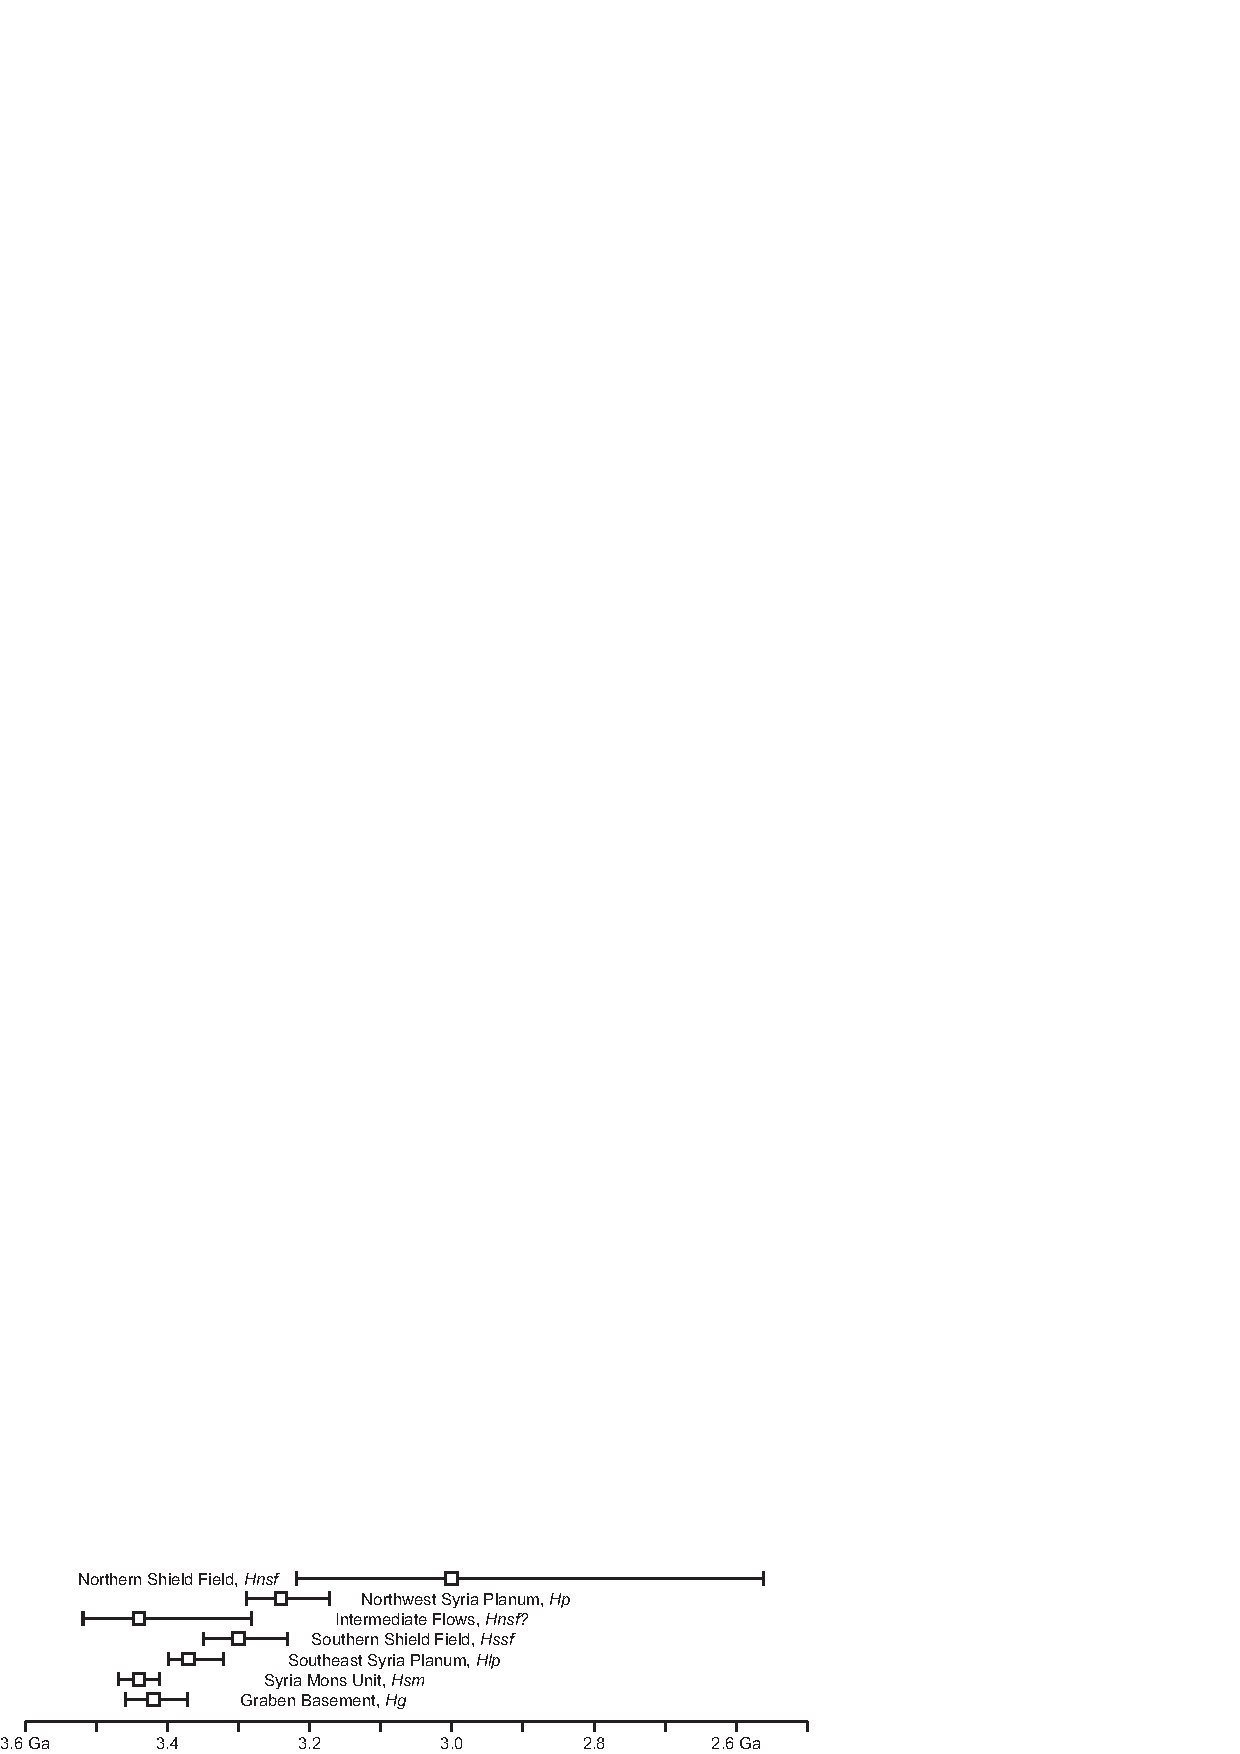
\includegraphics[width=\textwidth]{fig2.pdf}
\caption[A typical TRI field setup at Brei{\dh}amerkurjökull.]{A typical TRI field setup at Brei{\dh}amerkurjökull. The top antenna transmits at Ku-band (1.74 cm wavelength) and the bottom two antennas receive the backscattered signal. The antenna mount scans in azimuth, in this area up to 100$^{\circ}$. The calving front is approximately 4~km away. Note icebergs in the foreground.}
\label{fig:fieldsetup}
\end{figure*}


\begin{figure*}
\centering
%\includegraphics[width=178mm]{tsx_tri_figure/fig1.pdf}
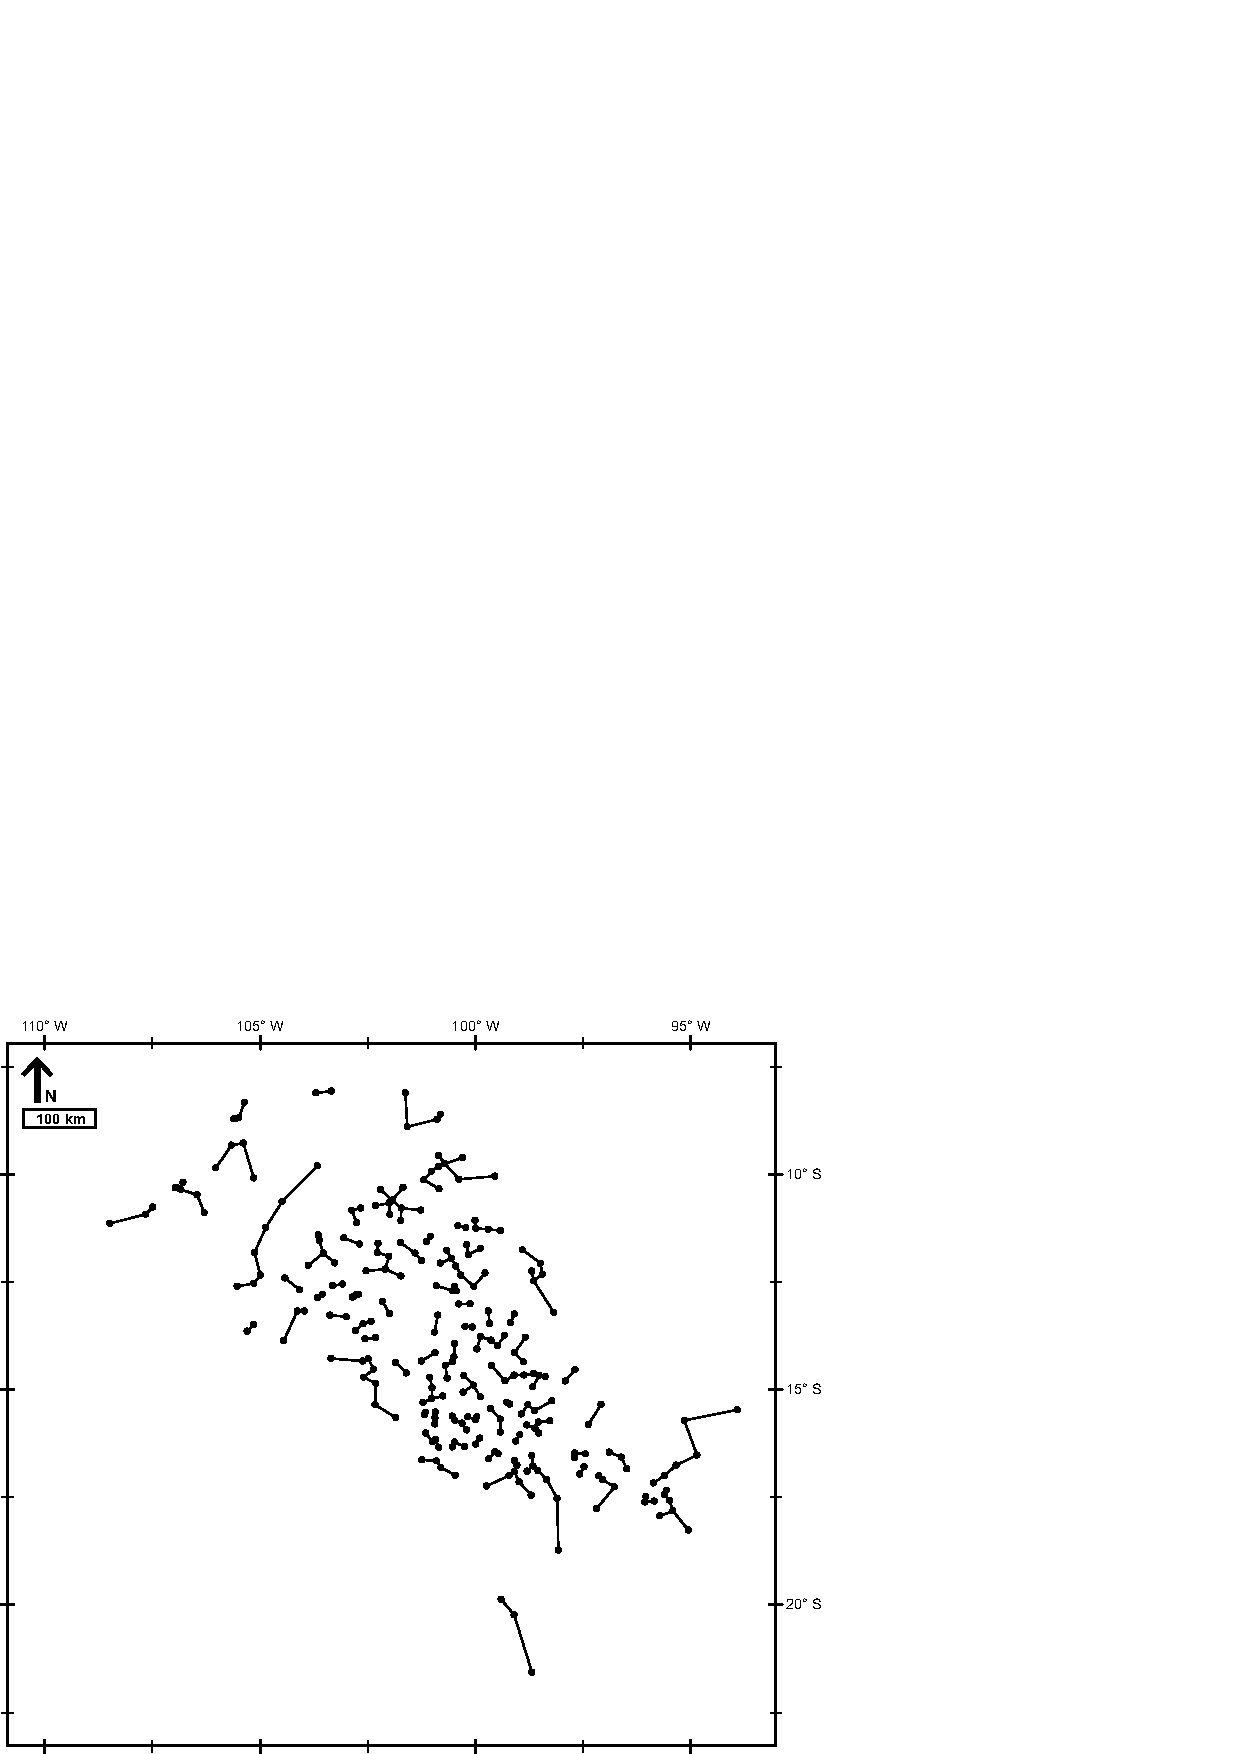
\includegraphics[width=\textwidth]{fig3.png}
\caption[2011-2013 velocity maps obtained using TRI (left) and TerraSAR-X (right).]{2011-2013 velocity maps obtained using TRI (left) and TerraSAR-X (right). Both TRI and TerraSAR-X velocities were adjusted to match the direction of ice motion (140$^{\circ}$ clockwise from north) using Equation 3. Note the similarity in velocity magnitude and distribution between the TRI and satellite maps despite the different acquisition and averaging times (3.5 hours for the TRI vs 11 days for TerraSAR-X).}
\label{fig:velmaps}
\end{figure*}

\begin{figure*}
\centering
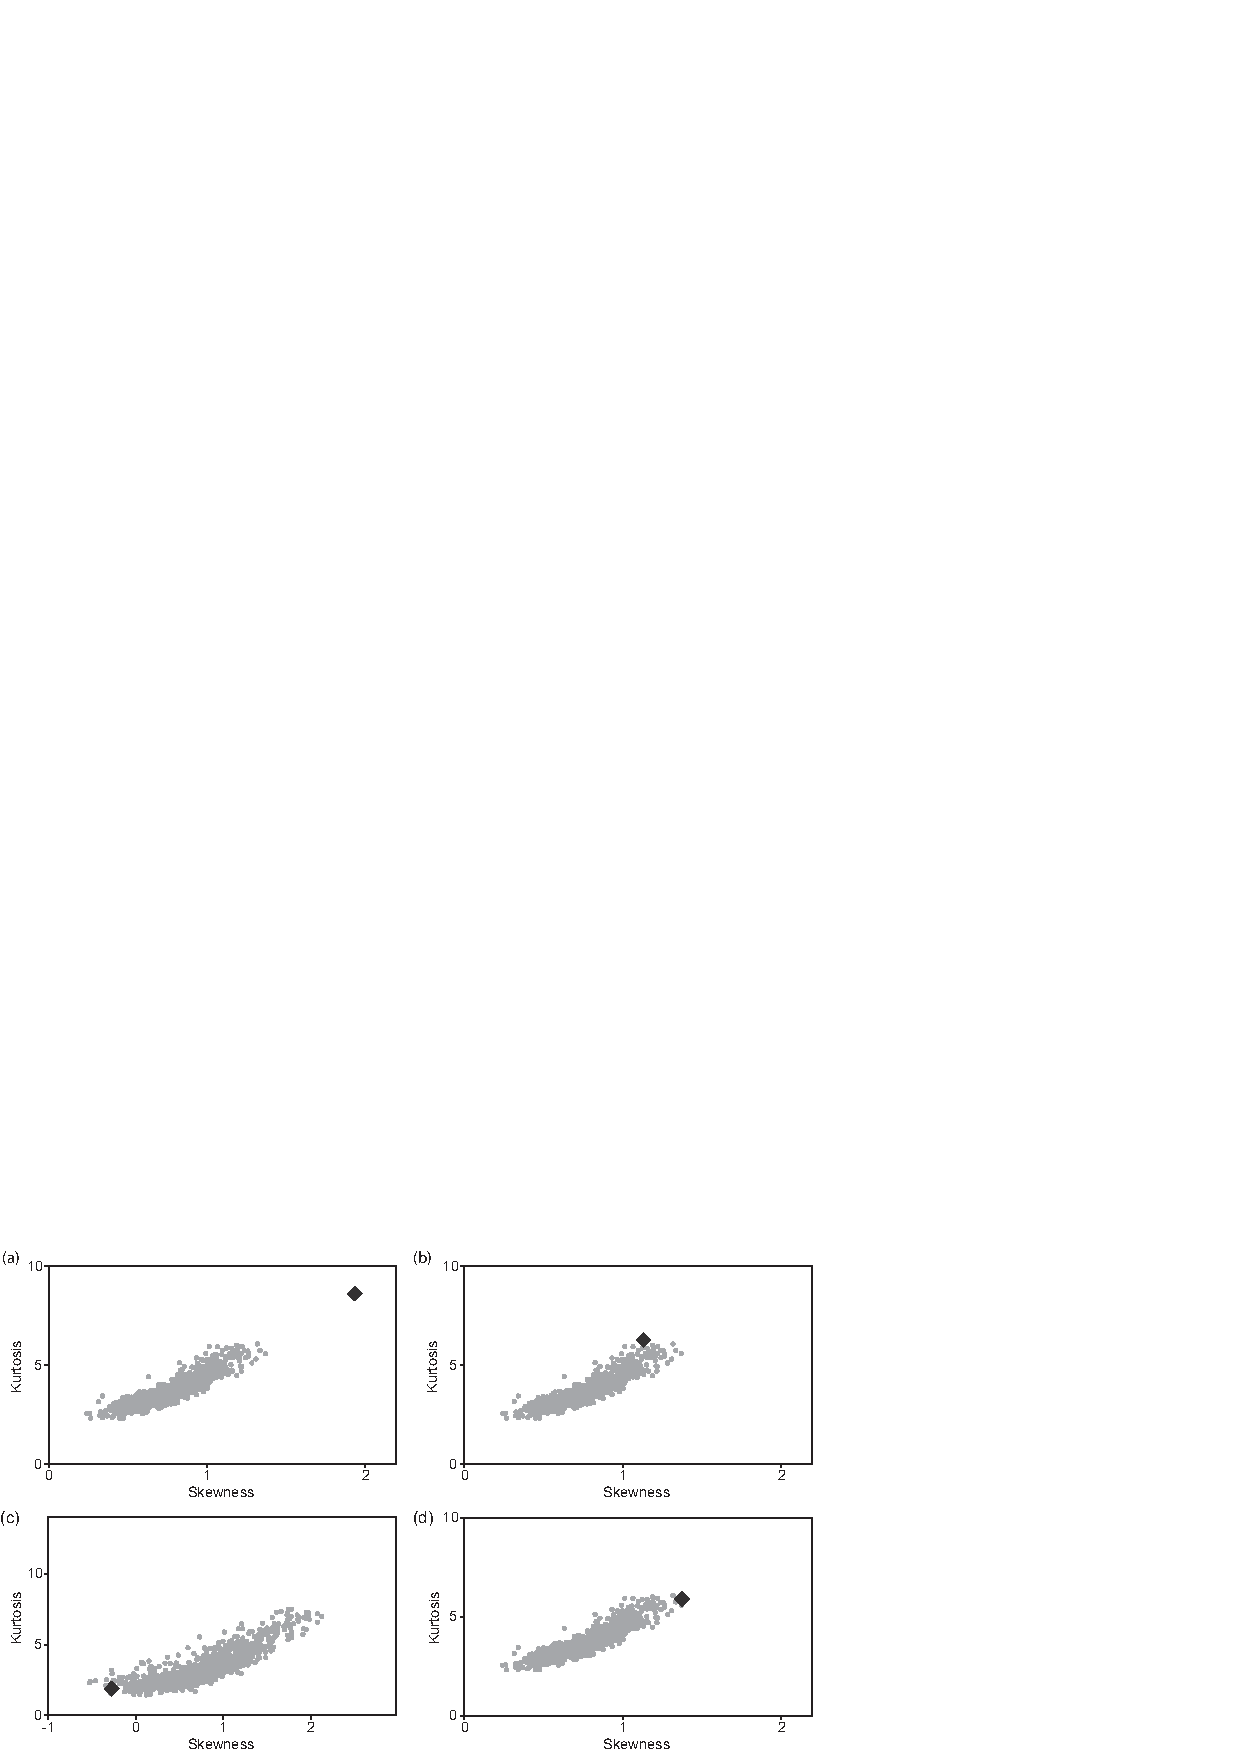
\includegraphics[width=\textwidth]{fig4.png}
\caption[Differences between the TerraSAR-X and TRI velocity maps in the direction of ice motion.]{Differences between the TerraSAR-X and TRI velocity maps in the direction of ice motion. Despite different sampling periods (11 days vs 3.5 hours), the agreement between the TRI and TerraSAR-X is reasonable (rms difference of  \textasciitilde1~m/d for all years) except for areas near crevasses and a small region near the highly-dynamic terminal zone.}
\label{fig:velmapserror}
\end{figure*}



% \pagebreak
\begin{figure*}
\centering
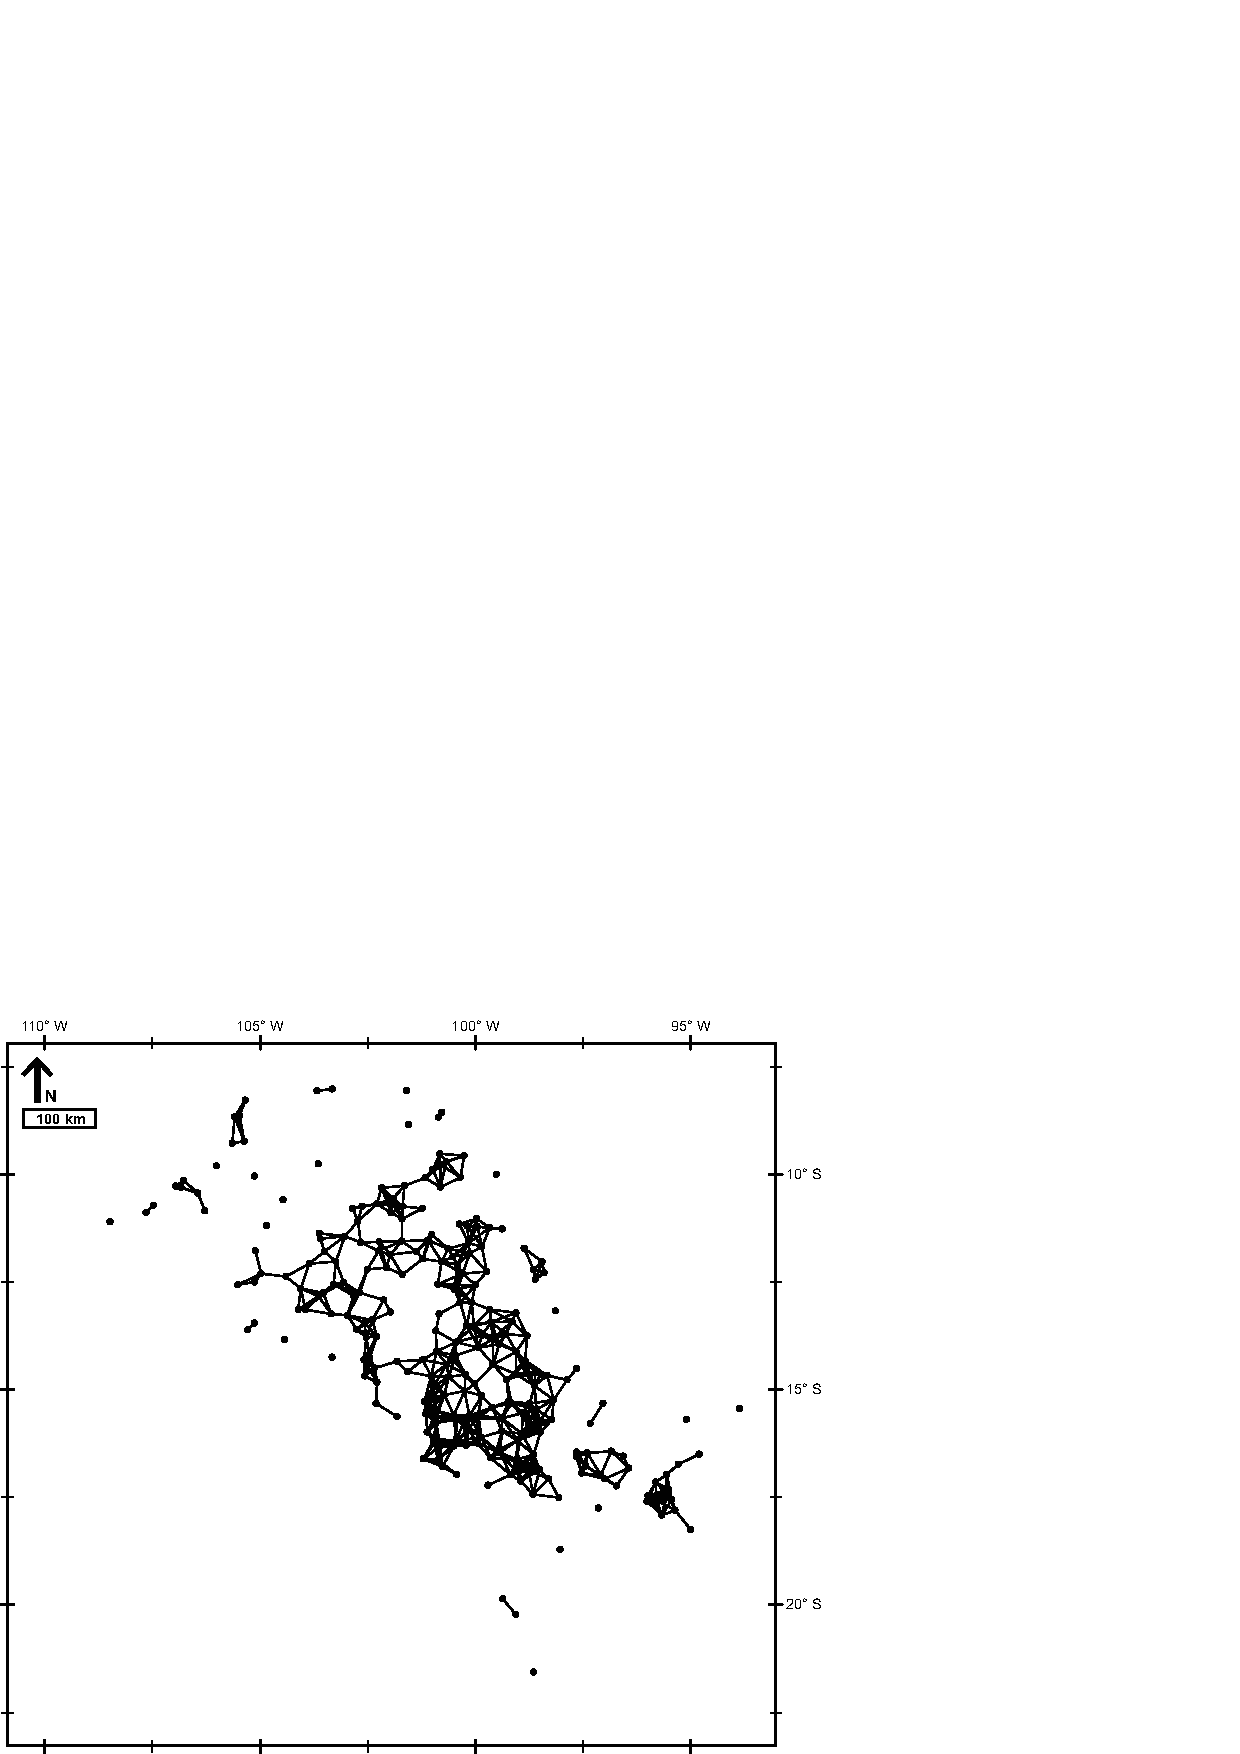
\includegraphics[width=\textwidth]{fig5.png}
\caption[Differences between the TerraSAR-X and TRI velocity maps in the direction of ice motion.]{
Terminus outlines from TRI and LANDSAT for the period 2008-2013, and the location of points discussed in the paper. Displacement (v) and noise (n) time series points from 2011 and 2012 are shown along with the BSOP/CTD locations. Points v1, v2, and v3 are velocity measurements from 2012 located on the moving ice. Points n1, n2, and n3 are stationary areas used to assess noise characteristics in 2012. Point n1 is located on moraine
deposits near the lagoon shore. Point n2 is located on a mountain. Point n3 is located on
stagnant ice near a medial moraine. Points 1, 2, and 3 show the locations on the ice selected for tidal comparisons in 2011. The marked lines show the terminus positions and embayment dynamics observed by LANDSAT and TRI. Note that the embayment opens during the summer of 2012 and 2013, and partially closes during the winter/spring of 2013 and 2014. }
\label{fig:12tslocs}
\label{fig:11tidelocs}
\label{fig:retreat}
\end{figure*}

% \pagebreak
\begin{figure*}                  
\centering
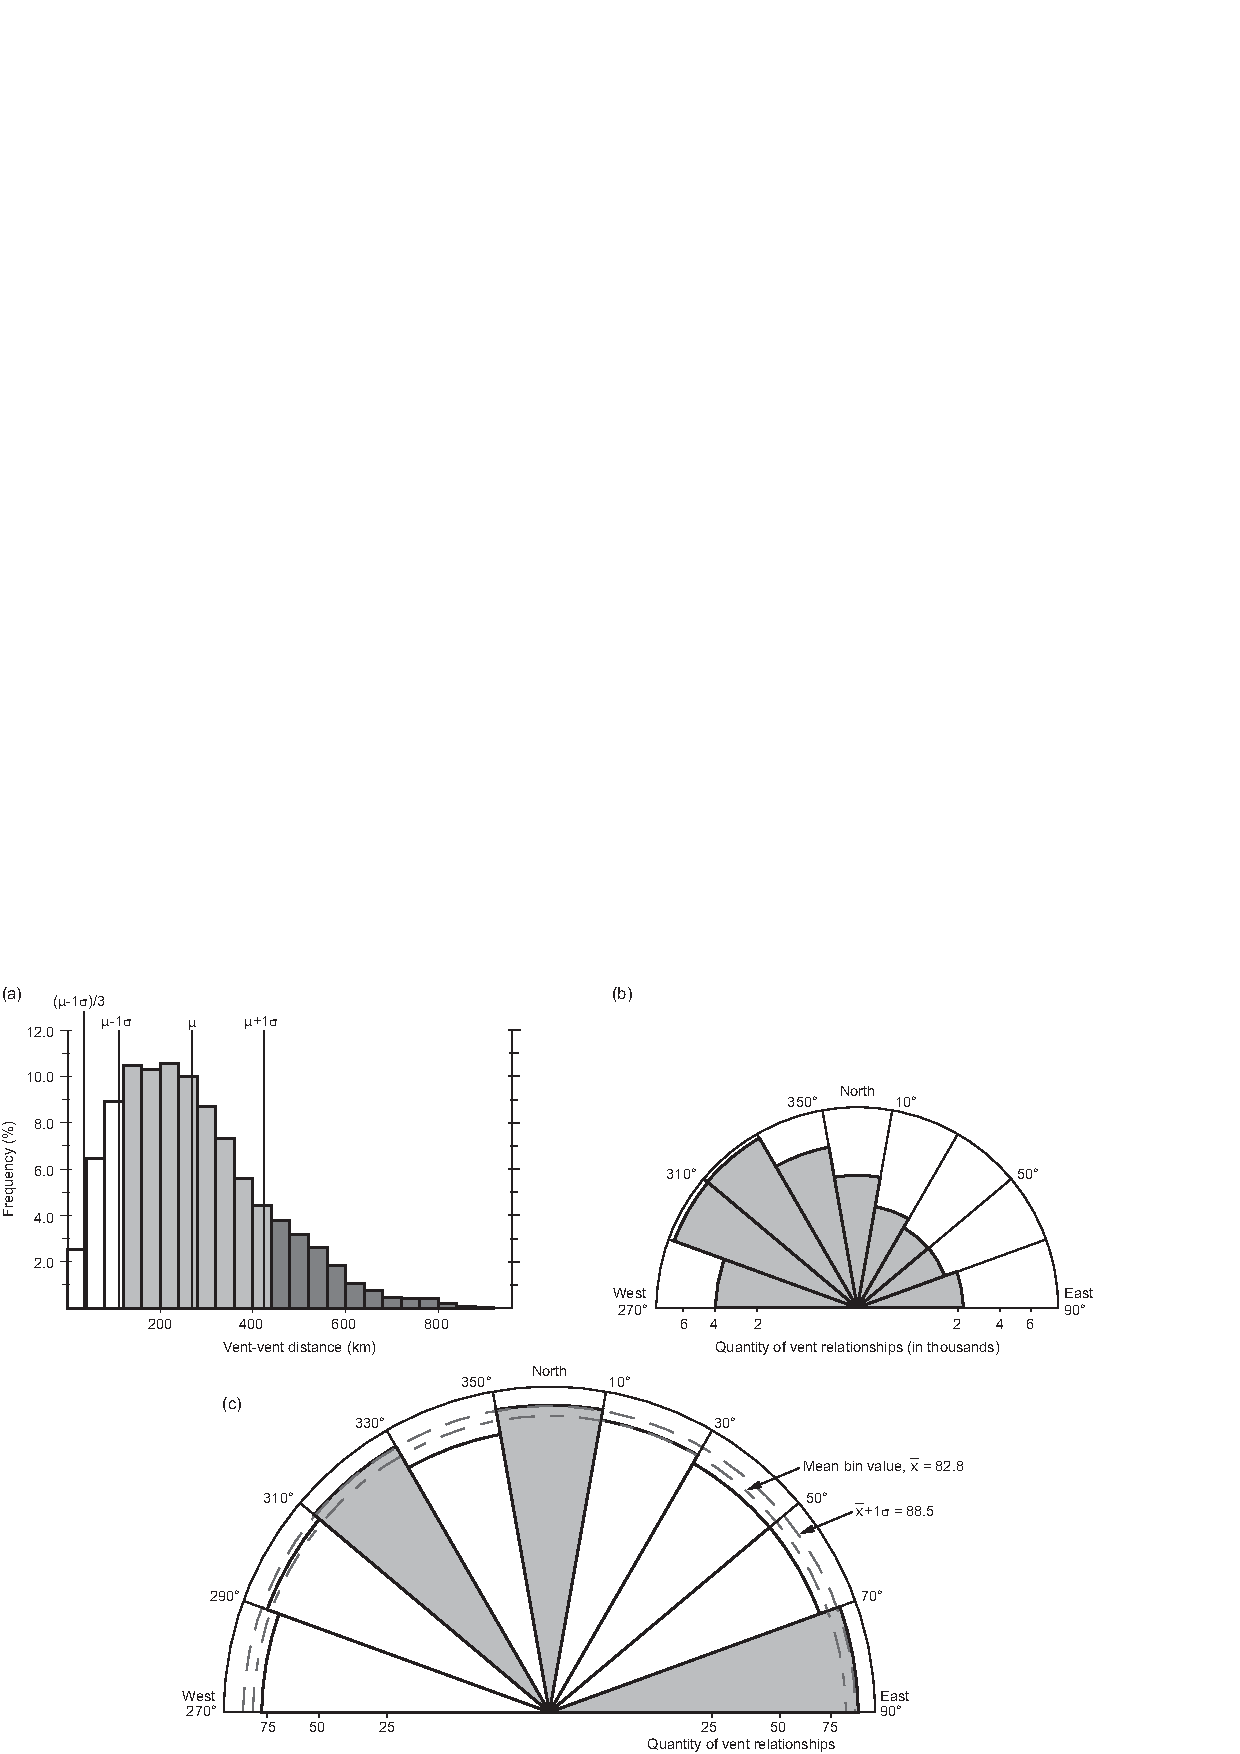
\includegraphics[width=\textwidth]{fig6.pdf}       
\caption[Displacement time series, 2012, for the points shown in Figure \ref{fig:12tslocs}.]{Displacement time series, 2012, for the points shown in Figure \ref{fig:12tslocs}. A (top) shows actual displacement, B (bottom) shows detrended displacement. Labels in the top panel show the location, the distance from the radar, the best-fit velocity, and the rms uncertainty for the three points on the glacier. Variations in velocity and rms scatter are related to distance from the glacier terminus (velocity and rms scatter decrease with increasing distance)}
\label{fig:ts12}
\end{figure*}

% \pagebreak
\begin{figure*}         
\centering
\includegraphics[width=\textwidth]{fig7.pdf}       
\caption[Similar to Figure \ref{fig:ts12}, displacement time series, 2012, for stationary targets (a measure of noise).]{Similar to Figure \ref{fig:ts12}, displacement time series, 2012, for stationary targets (a measure of noise). Location of points shown in Figure \ref{fig:12tslocs}. A (top) shows the actual displacement. B (bottom) shows the detrended displacement. Labels in the top panel show the point location, distance from the radar, linear velocity, and rms displacement from zero.}
\label{fig:nzts12}
\end{figure*}

% % \pagebreak
% \begin{figure} 
% \centering 
% \includegraphics[trim= .2cm .2cm .2cm .2cm, clip=true,width=86mm]{new_figures/2011tidelocs.pdf}
% \caption{Locations on the ice selected for tidal comparisons, 2011.}
% \label{fig:11tidelocs}
% \end{figure}



% \pagebreak
\begin{figure*}
\centering
\includegraphics[width=\textwidth]{fig8.pdf}
\caption[A comparison of theoretical rate error (Equation 7) to line-of-sight velocity uncertainties for different averaging times for the stationary points shown in Figure \ref{fig:12tslocs}.]{A comparison of theoretical rate error (Equation 7) to line-of-sight velocity uncertainties for different averaging times for the stationary points shown in Figure \ref{fig:12tslocs}.}
\label{fig:12error}
\end{figure*}

% \pagebreak
\begin{figure*}               
\centering
\includegraphics[width=\textwidth]{fig9.pdf}        
\caption[Displacement and tide time series, 2011.]{Displacement and tide time series, 2011. Top panel shows total displacement for three points (Figure \ref{fig:12tslocs}) and tides (black line). Bottom panel shows detrended displacement and tides. Small calving events can be seen in the tidal record. There are no apparent velocity variations associated with the tidal signal over the short acquisition period, but longer time series are necessary for a more thorough analysis.}
\label{fig:11tidedisp}
\end{figure*}





% % \pagebreak
% \begin{figure}
% \centering
% %\includegraphics[trim= .2cm .2cm .2cm .2cm, clip=true, width=86mm]{new_figures/retr.pdf}
% \includegraphics[trim= .2cm .2cm .2cm .2cm, clip=true, width=86mm]{termmap.pdf}
% \caption{Terminus retreat and embayment dynamics observed by LANDSAT and TRI. Note the formation, closing, and reappearance
% of the embayment in 2008, 2012, and 2013.}
% \label{fig:retreat}
% \end{figure}

% \pagebreak
\begin{figure*}
\centering
\includegraphics[width=\textwidth]{fig10.png}
\caption[A perspective view of the smoothed TRI-derived DEMs in 2011 and 2012, and their difference.]{A perspective view of the smoothed TRI-derived DEMs in 2011 and 2012, and their difference. There is substantial ice loss immediately adjacent to the terminus.}\label{fig:dems}
\label{fig:demperspective}
\end{figure*}






% \pagebreak
\begin{figure*}
\centering
\includegraphics[width=\textwidth]{fig11.png}
\caption[Map of ice loss between 2011 and 2012.]{Map of ice loss between 2011 and 2012. Note that most of the ice was lost in the region around the seasonal embayment. The colored boxes show the areas used for ASTER/TRI DEM comparisons (yellow) and the 2011-2012 TRI DEM comparisons (cyan).}
\label{fig:dems}
\end{figure*} 


\begin{figure*}
\centering
\includegraphics[width=\textwidth]{fig12.pdf}
\caption[Smoothed line-of-sight velocity and elevation profiles in the vicinity of the terminus along the center line of the imaged area in 2011 and 2012.]{Smoothed line-of-sight velocity and elevation profiles in the vicinity of the terminus along the center line of the imaged area in 2011 and 2012. The inset at the top left shows the approximate surface slopes near and upglacier of the ice cliff.}
\label{fig:velelev}
\end{figure*}


\begin{figure*}
\centering
\includegraphics[width=\textwidth]{fig13.png}
\caption[Counterclockwise iceberg motion through the embayment in 2012.]{Counterclockwise iceberg motion through the embayment in 2012. This kind of circulation may represent horizontally partitioned flow, where surface and near surface lagoon waters flow into the embayment and circulate in a counterclockwise direction with fast velocities. Here, the iceberg enters the embayment at a speed of \textasciitilde6 cm/s, accelerates to \textasciitilde18 cm/s as it passes through, and slows down to \textasciitilde7~cm/s as it exits the embayment on the other side into the open water. This suggests that there may be high fluxes of water passing through the embayment.}
\label{fig:icemotion}
\end{figure*}


\begin{figure*}
\centering
%MANUALLY FIX THIS ONE
\includegraphics[width=.5\textwidth]{fig14.png}
\caption[A five-hour period showing an outflow event observed in 2012.]{A five-hour period showing an outflow event observed in 2012. Such outflow events may represent vertically partitioned flows where cold, fresh meltwater emerges from the base of a glacier, rapidly rises to the surface and flows outward as a broad, shallow surface current pushing out  the nearby icebergs. The iceberg closest to the center of the lagoon (cyan) gets pushed away from the vicinity of the terminus. Note the slower speed and the clockwise trend shown by the icebergs (circled in red and yellow) that are less affected by the outflow event.}
\label{fig:OFQ}
\end{figure*}


% \pagebreak
\begin{figure*}
\centering
\includegraphics[width=\textwidth]{fig15.png}
\caption[Lagoon salinity and temperature profiles from the 2012 BSOP deployment and the 2013 CTD casts showing that Jökulsárlón is well-mixed with only slightly warmer, saltier 
water at the bottom.]{Lagoon salinity and temperature profiles from the 2012 BSOP deployment and the 2013 CTD casts showing that Jökulsárlón is well-mixed with only slightly warmer, saltier 
water at the bottom. The data consist of multiple casts (to various depths) for each instrument. The cast locations are shown in Figure \ref{fig:retreat}, and illustrate some of the depth variability within the lagoon. The CTD locations were closer to the deeper central portion of the lagoon, while the BSOP locations were closer to shore. Small outlying points may be related to the CTD hitting the lagoon bottom.}
\label{fig:ctd}
\end{figure*}


\begin{figure*}
\centering
%\includegraphics[width=86mm]{new_figures/mixplots.pdf}
\includegraphics[width=\textwidth]{fig16.png}
\caption[BSOP and CTD data showing the mixed properties of the lagoon water in comparison to two linear mixing models.]{BSOP and CTD data showing the mixed properties of the lagoon water in comparison to two linear mixing models. The two endmember waters appear to be a 0$^{\circ}$C, 0 psu salinity freshwater and an ocean water with temperature between 4 and 6$^{\circ}$C and salinity 35 psu (warmer temperatures in the upper left reflect atmospheric warming in the top 5 meters). A Gade line with a typical slope of 2.5$^{\circ}$C/psu is shown, suggesting that late-summer measurements are not significantly affected by ocean-forced melting. Outliers below a salinity of 1 were discarded.}
\label{fig:mplots}
\end{figure*}






% \end{document}

% \documentclass[review]{elsarticle}
% 
% \usepackage{lineno,hyperref}
% \usepackage{amsmath}
% \usepackage{graphicx}
% 
% 
% %support icelandic fonts
% \usepackage[T1]{fontenc}
% \usepackage{lmodern} %this is needed with T1
% \usepackage[utf8]{inputenc}  
% 
% 
% \modulolinenumbers[5]
% 
% \journal{Computers \& Geosciences}
% 
% %%%%%%%%%%%%%%%%%%%%%%%
% %% Elsevier bibliography styles
% %%%%%%%%%%%%%%%%%%%%%%%
% %% To change the style, put a % in front of the second line of the current style and
% %% remove the % from the second line of the style you would like to use.
% %%%%%%%%%%%%%%%%%%%%%%%
% 
% %% Numbered
% %\bibliographystyle{model1-num-names}
% 
% %% Numbered without titles
% %\bibliographystyle{model1a-num-names}
% 
% %% Harvard
% %\bibliographystyle{model2-names.bst}\biboptions{authoryear}
% 
% %% Vancouver numbered
% %\usepackage{numcompress}\bibliographystyle{model3-num-names}
% 
% %% Vancouver name/year
% %\usepackage{numcompress}\bibliographystyle{model4-names}\biboptions{authoryear}
% 
% %% APA style
% \bibliographystyle{model5-names}\biboptions{authoryear}
% 
% %% AMA style
% %\usepackage{numcompress}\bibliographystyle{model6-num-names}
% 
% %% `Elsevier LaTeX' style
% % \bibliographystyle{elsarticle-num}
% % \bibliographystyle{model2-names}
% %%%%%%%%%%%%%%%%%%%%%%%
% 
% %way to avoid long lines for function names
% \pretolerance=10000
% 
% \begin{document}
% 
% \begin{frontmatter}

% \title{Current observations in a proglacial lagoon in southeastern Iceland with automated iceberg tracking and Terrestrial Radar Interferometry}
% \title{Lagoon current observations in southeastern Iceland with automated iceberg tracking and Terrestrial Radar Interferometry}

\chapter[Observations of Inertial Currents in a Lagoon in Southeastern Iceland Using Terrestrial Radar Interferometry and Automated Iceberg Tracking]{Observations of Inertial Currents in a Lagoon in Southeastern Iceland Using Terrestrial Radar Interferometry and Automated Iceberg Tracking \footnote{This chapter is in review as: Voytenko, D., Dixon, T. H., Howat, I. M., Luther M., Lembke, C., de la Peña, S., Lagoon current observations in southeastern Iceland with automated iceberg tracking and terrestrial radar interferometry, Computers and Geosciences.}}


% \chapter[Observations of inertial currents in a lagoon in southeastern Iceland using terrestrial radar interferometry and automated iceberg tracking]{Observations of inertial currents in a lagoon in southeastern Iceland using terrestrial radar interferometry and automated iceberg tracking \footnote{This chapter is in review as: Voytenko, D., Dixon, T. H., Howat, I. M., Luther M., Lembke, C., de la Peña, S., Lagoon current observations in southeastern Iceland with automated iceberg tracking and terrestrial radar interferometry, Computers and Geosciences.}}

% \tnotetext[mytitlenote]{Fully documented templates are available in the elsarticle package on \href{http://www.ctan.org/tex-archive/macros/latex/contrib/elsarticle}{CTAN}.}

%% Group authors per affiliation:
% \author{Denis Voytenko\fnref{myfootnote}}
% \author{Denis Voytenko\fnref{fn1}}
% \fntext[fn1]{Corresponding author. dvoytenk@mail.usf.edu, 813-508-8486}

% \corauth[cor]{Corresponding author. 813-508-8486}

% 
% \author{Timothy H. Dixon}
% \address{School of Geosciences, University of South Florida, Tampa, Florida, USA.}
% \author{Ian M. Howat}
% \author{Santiago de la Peña}
% \address{School of Earth Sciences and Byrd Polar Research Center, The Ohio State University,
% Columbus, Ohio, USA.}
% \author{Chad Lembke}
% \author{Mark E. Luther}
% \address{College of Marine Science, University of South Florida, St. Petersburg, Florida, USA.}
% % \fntext[myfootnote]{Since 1880.}
% 
% % %% or include affiliations in footnotes:
% % \author[mymainaddress,mysecondaryaddress]{Elsevier Inc}
% % \ead[url]{www.elsevier.com}
% % 
% % \author[mysecondaryaddress]{Global Customer Service\corref{mycorrespondingauthor}}
% % \cortext[mycorrespondingauthor]{Corresponding author}
% % \ead{support@elsevier.com}
% % 
% % \address[mymainaddress]{1600 John F Kennedy Boulevard, Philadelphia}
% % \address[mysecondaryaddress]{360 Park Avenue South, New York}

\section{Abstract}
Ocean currents are considered to be a contributing factor to the retreat of marine-terminating glaciers worldwide, but direct observations near the ice-ocean interface are challenging. We use radar intensity imagery and an iceberg tracking algorithm to produce half-hourly current maps within an imaged portion of Jökulsárlón, a proglacial lagoon in southeastern Iceland. Over our 43.5-hour observation period, the lagoon has clockwise circulation with current speeds of order 3-8 cm/s and occasional strong glacier outflows of up to \textasciitilde 15 cm/s. The currents are dominantly inertial, driven by the glacial outflows.
% \end{abstract}

% \begin{keyword}
% Terrestrial Radar Interferometry, iceberg tracking, inertial currents
% \end{keyword}
% 
% \end{frontmatter}
% 
% \linenumbers

\section{Introduction}
\subsection{Overview}
Sea ice monitoring programs and automated iceberg tracking algorithms have been used in maritime operations to prevent damage to ships or oil rigs \citep{smith1983influence}.   Many of these programs and algorithms involve imaging radar, because of its day/night, all-weather capability. Here we use radar intensity imagery, in conjunction with a new automated iceberg tracking algorithm, to develop insights into the hydrography of a proglacial lagoon.

Improved knowledge of ice-ocean interactions is important for predicting the behavior of marine-terminating (tidewater) glaciers, many of which are presently undergoing rapid retreat \citep{straneo2013challenges}. The role of ocean circulation in melting and calving of marine-terminating glaciers has been recognized for some time \citep{motyka2003submarine,holland2008acceleration,straneo2010rapid}.  However, details of this circulation process in the immediate vicinity of the glacier terminus remain obscure because the possibility of iceberg calving makes direct observation dangerous.   

GPS receivers have been emplaced on icebergs for current monitoring \citep{sutherland2014quantifying}. Remotely-sensed imagery may be useful in fjords and lagoons where iceberg motion can be used to track surface and near-surface currents.  Here we report results based on imagery acquired with a Terrestrial Radar Interferometer (TRI). A TRI is a ground-based instrument designed to monitor small-scale displacements on the glacier's surface with high sampling rate and precision using interferometry based on phase comparisons of successive images \citep{voytenko2014}.  However, instead of using phase interferometry to measure the speed of glacier ice, here we exploit the intensity imagery and the high sampling rate of the system. Unlike the motion of the glacier ice, smaller icebergs in proglacial lagoons tend move too fast to be tracked interferometrically, so intensity-based tracking is required. 

% % IMPROVE PTV/PIV DISCUSSION. 
% Although visual tracking methods have been extensively studied and applied to a variety of fields (e.g. Particle Image (PIV) and Tracking Velocimetry (PTV) \citep{dracos1996particle,adrian2005twenty}), including 

There are two commonly used methods for detecting motion in imagery: Particle Image Velocimetry (PIV) and Particle Tracking Velocimetry (PTV).
PIV is based on measuring the motion of blocks of the image containing numerous particles, while PTV focuses on tracking particles individually. These methods have been extensively studied and applied to a variety of fields including river gauging \citep{creutin2003river} and iceberg tracking from satellite imagery over long time steps \citep{silva2005computer}.

In this study,  we focus on a PTV approach for tracking icebergs over several minute time steps.  First, we use the intensity of the backscattered signal to find the positions of icebergs in the lagoon, whose centroids are detected using a connected component labeling algorithm. Second, we track the iceberg positions in time using a nearest-neighbor approach and generate the resulting velocity maps using radial basis function (RBF) interpolation. This method has been successfully used for surface, image, and topographic reconstruction \citep{hardy1971multiquadric,carr1997surface,carr2001reconstruction,gumerov2007fast},  to infer the behavior of the lagoon currents.


\subsection{Site setting}
Jökulsárlón is a tidal lagoon at the terminus of Brei{\dh}amerkurjökull, an outlet glacier of Vatnajökull, Iceland's largest ice cap (Figure \ref{fig:map}). The lagoon has an area of \textasciitilde20 $km^2$, a maximum depth of around 300~m, and is connected to the North Atlantic Ocean via a narrow, engineered, channel \citep{bjornsson1996scales,bjornsson2001jokulsarlon,howat2008dynamic}. Brei{\dh}amerkurjökull occasionally calves icebergs into Jökulsárlón. We track these icebergs in this study.  

The hydrodynamics of this lagoon appear to be complicated, as there are several sources or drivers of potential currents.  The lagoon is bounded by mountains on the east and west sides, a glacier on the north side, and the Atlantic Ocean on the south side. The glacier and the ocean bring in strong winds from opposing directions, while ocean tides modulate the currents near the narrow outlet to the ocean. The bounding glacier to the north also subjects the lagoon to calving-driven flows and subglacial drainage. 

The lagoon contains both cold, fresh, meltwater from the glacier, and  warm, saline, water from the Atlantic ocean.  The salinity and temperature of the lagoon vary seasonally: 7-17 psu with temperatures between 1 and 5~deg.~C in the summer \citep{DIXONEOS} and 15-21 psu with temperatures between 0.5 and 2 $^\circ$ C in the spring \citep{brandon2013hydrographic}. Winter measurements are not available.

\section{Methods}


\subsection{Data acquisition}
We used a GAMMA Portable Radar Interferometer as the TRI instrument for this study \citep{werner2008real}. This is a Ku-band, real-aperture radar with a range resolution of 0.75 m and an azimuth resolution of 7.5 m at 1 km. The azimuth resolution decreases linearly with distance (e.g., 15~m at 2~km). We deployed the TRI in August of 2012 covering 90-degree arcs with a range of 50 m to 8.5 km and a two minute sampling rate (an ideal sampling rate for measuring rapid iceberg motion in this lagoon). 

Since the primary purpose of the TRI is to monitor ice surface velocities, the TRI must be set up with a clear view of both the pro-glacial lake and of the glacier to measure ice surface velocities and to track the icebergs (Figure \ref{fig:radar}). We created 87 current maps during our observation period spanning a continuous 43.5-hour period.

During the study period, we also deployed an autonomous CTD (conductivity-temperature-depth) profiler, specifically a bottom-stationed ocean profiler (BSOP) \citep{langebrake2002design} in the lagoon (Figure \ref{fig:tsplot}). During one three-hour period, the BSOP was untethered and moved with the surface currents while continually logging its position (Figure \ref{fig:map}). We used the BSOP position data over this period to verify the current maps and speeds derived from our iceberg tracking algorithm.


The iceberg detection and tracking scripts were written in Python using SciPy, NumPy and Matplotlib \citep{hunter2007matplotlib, oliphant2007python}. The intensity imagery and the processing scripts are available on GitHub.


\subsection{Radar pre-processing}
Intensity images are extracted from the radar data and converted to map coordinates with 10~m pixel spacing using the GAMMA software package. The icebergs are detected sequentially image-by-image. Before detection, each image is pre-processed (Figure \ref{fig:preproc}). The pre-processing is responsible for removing speckle and simplifying iceberg detection. This step is facilitated by the basic characteristics of the radar intensity images. The icebergs act as strong radar scatterers, appearing bright in the image, while the water surface reflects most of the radar energy away from the instrument, and hence appears dark in the image.

The first step in the pre-processing procedure is masking. The mask is the area containing the boundaries of the lagoon, and any pixels outside of the mask are not considered to be an iceberg and are discarded. Once the lagoon is selected, the process focuses on minimizing noise (unfortunately, small icebergs may also be removed in this step).  This is accomplished with a sequence of a Gaussian blur ($\sigma=1$), a threshold ($0.3$), another Gaussian blur ($\sigma=1$) and another threshold ($0.3$). 

The thresholding operation creates a binary image, as any pixel value above the threshold criterion is converted to a 1, and every other pixel to a 0. The final image that undergoes iceberg detection is thus a binary image where each pixel is either a part of an iceberg (foreground) or a part of the lagoon (background).

\subsection{Iceberg detection}
Each iceberg in the binary image is detected with a connected-component labeling algorithm. The purpose of this algorithm is to identify, and uniquely label, individual components of the image that are only connected to themselves, and distinguish them from other discrete components. We use the SciPy implementation of the two-pass connected component algorithm (scipy.ndimage.measurements.label) based on the classical algorithm proposed by \citet{rosenfeld1966sequential}. 

An illustration of the connected component algorithm is shown in Figure \ref{fig:cca}. The image is scanned line-by-line, and border pixels are set to the background value. The first pass over the image labels each pixel in a specific way. If the pixel is a foreground (iceberg) pixel, the algorithm checks to see if any of the four of its neighbors (W, NW, N, NE pixels) are also foreground pixels. Once that check is complete, there are three possibilities: 1) if no neighbors are in the foreground, the pixel is given a new label; 2) if only one of the neighboring pixels is in the foreground, then the pixel is given the same label as the other foreground neighbor pixel; 3) if two or more neighboring pixels are in the foreground, then the pixel is assigned a label of either of the foreground neighboring pixels. When this happens, the algorithm stores that all of the labels seen in this step are equivalent. 
Once all of the pixels have been successfully labeled, the second pass over the image resolves the equivalence between labels: every pixel that belongs to the same set of equivalent pixels is given the same label. Subsequently, all icebergs are relabeled in a consecutive order.

Once every iceberg is given its own label, we find the positions of every pixel with the same label in every iceberg, and calculate the centroid of each iceberg, keeping that information for later tracking. The centroid of an iceberg is the average $x$ and $y$ positions of all its constituent pixels, and is compared from image to image the tracking. The algorithm moves on to the next image, and repeats. Once the centroids for every detected iceberg in every image are found, we begin the tracking process.

\subsection{Iceberg tracking}
The tracking algorithm is based on a nearest-neighbor approach. The first image initializes the centroids of icebergs detected (these are the icebergs that are going to be tracked). Then, for every new image, the locations of the centroids in the image are compared to the locations of the centroids in the previous image. We specify a maximum distance (20~m for for this study) and find the closest centroid in the new image. This is repeated iteratively, giving a time series of iceberg centroid positions, which can be converted into the velocities. Icebergs that are not detected (e.g., if they become shadowed for one acquisition) are assigned the coordinates from the previous time step.

\subsection{Current map generation}
Although data are available for every measurement, we linearize the motion over a 30 minute time step to account for noise and for temporarily-undetected icebergs. No new icebergs are introduced into the system over this period. Two positions are used to calculate the velocity, one at the beginning (0 minutes) and one at the end (30 minutes). Icebergs that moved less than 2 pixels over the half-hour period (speed of 1 cm/s), are considered stationary and discarded. Since we can calculate a velocity for every iceberg at every 30-minute time step, we can specify those velocities at the last known locations of the icebergs and interpolate maps representing the $x$ and $y$ components of velocity. 


Since iceberg motion measurements are relatively sparse, the $x$ and $y$ velocities are interpolated onto a 25x25 grid using a linear radial basis function (RBF) interpolation in SciPy.  Each velocity component is interpolated separately.

The RBF interpolation solves for the velocity component at each grid point by depending on velocity values from every measurement point weighted by the distances to that point.




The general equation for the RBF interpolation is \citep{buhmann2003radial}:
%\begin{equation}s(x)=\sum\limits_{i=1}^N \lambda_\phi(||x-x_i||)+P(x)\end{equation}
\begin{equation}s(x)=\sum\limits_{i=1}^N \lambda_i\phi(||p-p_i||)\end{equation}
where $s(x)$ is the velocity of the interpolated point, $\lambda_i$ is a weight coefficient, $\phi$ is the radial basis function, $p$ is the interpolation point, and $p_i$ is a data point.

Although there are many types of radial basis functions, the linear RBF has a simple form
\begin{equation}\phi(r)=r\end{equation}
where $r$ is the radius from the interpolated point to a data point.

However, for our purposes, we can rewrite the general interpolation equation as
\begin{equation}v(r)=\sum\limits_{j=1}^N\lambda_j\phi(r)\end{equation}
%
where $v$ is the interpolated velocity, $i$ is an index of an interpolated point, $\phi(r)$ is the RBF, which depends on the radius, and $j$ is the index of a data point. Therefore, the velocity at a point that is interpolated depends on the velocities of all of the available data points and their respective distances to the interpolated point.

Although we have a general equation for the interpolation, we still need to calculate the $\lambda$ coefficients, which are weights associated with the velocities of the data points and their distances to each other. The $\lambda$ coefficients are computed by solving a system of linear equations
\begin{equation}\mathbf{\lambda}=A^{-1}\mathbf{v}\end{equation}

where $\lambda$ is the vector of weights associated with the distances related to the data points, $A$ is a Euclidian Distance Matrix (EDM) describing the distances between points in a specific format, and $v$ is a vector of velocities of the known points. 
The format of the EDM is:
\begin{equation}\begin{bmatrix}
||p_1-p_1|| & ||p_1-p_2|| & \cdots & ||p_1-p_n||\\
||p_2-p_1|| & ||p_2-p_2|| & \cdots & ||p_2-p_n||\\
\vdots & \vdots & \ddots & \vdots \\
||p_n-p_1|| & ||p_n-p_2|| & \cdots & ||p_n-p_n||\\
\end{bmatrix}\end{equation}
where $p_i$ is a data point with coordinates $(x_i,y_i)$.

Once we have the coefficients, the velocity at a desired point is calculated as a function of the distance to all of the available data points, weighted by the calculated coefficients.

% \begin{equation}z(x_i,y_i)=\sum\limits_{j=1}^N\lambda_j\phi(r)\indent r=\sqrt{(x_j-x_i)^2+(y_j-y_i)^2} \indent \phi(r)=r\end{equation}
The components of the interpolated velocities are represented as arrows on the current maps (Figures \ref{fig:currents} and \ref{fig:comparison}).

\subsection{Uncertainty analysis and verification}

Uncertainties were estimated using a Monte Carlo simulation with 1000 runs to determine the sensitivity of the linear RBF interpolation method to data noise. We assumed that uncertainties in determining the $x$ and $y$ position of the iceberg centroid were independent, and added a randomly sampled uncertainty parameter (assuming a zero-mean normal distribution and a standard deviation of 1 pixel) to each set of initial and final position measurements, producing 1000 interpolated maps for each of the two components of iceberg motion. 



We plot error ellipses related to the measurement uncertainties given a set of $x$ and $y$ position vectors from the Monte Carlo simulation. First, we calculate the covariance matrix
\begin{equation}
 \Sigma= \left[
  \begin{array}{ c c }
     \sigma_{x}^{2} & \sigma_{xy} \\
     \sigma_{yx} & \sigma_{y}^{2} 
  \end{array} \right]
\end{equation}.

Subsequently, $\Sigma$ is decomposed into a set of eigenvalues ($\lambda$) and eigenvectors ($\xi$)
\begin{equation}
\lambda=
 \left[ \begin{array}{c}
     \lambda_1  \\
     \lambda_2
  \end{array} \right]
\xi=
 \left[ \begin{array}{ c c }
     \xi_{11} & \xi_{21} \\
     \xi_{12} & \xi_{22}
  \end{array} \right]
\end{equation}.

Then, we follow \citet{haug2012bayesian} to obtain the parametric equations for the error ellipse given a specific confidence interval $P_c$. For example, we can calculate the area of an ellipse ($C^2$) that would encompass 95 percent of the data by using the equation 
\begin{equation}
 C^2=-2\ln(1-P_c)
\end{equation}
and setting $P_c=.95$.


Next, we use the square root of this area to scale the ellipse axes, whose length depends on the eigenvalues, and whose orientation depends on the eigenvectors, and $\theta$, a parametric vector on $[0,2\pi]$. This creates a set of angles, defining points ($x_e (\theta)$, $y_e (\theta)$) to plot the full ellipse around the average $x$ and $y$ positions (Figure \ref{fig:ellipses}) 

\begin{equation}
\left[
\begin{array}{c}
x_e (\theta) \\ y_e (\theta)
\end{array}
\right]
=
\left[
\begin{array}{c}
\hat{x} \\ \hat{y}
\end{array}
\right]
+
\left[
\begin{array}{c}
\xi_{11}C\sqrt{\lambda_1}cos(\theta)+ \xi_{12}C\sqrt{\lambda_2}sin(\theta) 
\\ 
\xi_{21}C\sqrt{\lambda_1}cos(\theta)+ \xi_{22}C\sqrt{\lambda_2}sin(\theta)
\end{array}
\right]
\end{equation}
.

The Monte Carlo simulation results show the distribution of uncertainties for a subset of selected points in Figure \ref{fig:ellipses}.

The \textasciitilde7-30\% error in the current speeds (assuming speeds of 3-15~cm/s and a centroid detection error of 1~cm/s) also appears to be reasonable, considering that the TRI was not designed to monitor currents. However, since the visual centroid detection error remains the same regardless of current speeds, the relative uncertainty becomes high in areas with very slow currents (2 cm/s or less).

We verified our technique in two ways. First, by comparing one automatically-detected current map to a manually-detected one. Second, by comparing our measured to motion of the BSOP.

The first verification method focused on the accuracy of the iceberg detection. The manually-detected current map was created by visually identifying the initial and final centroid positions of 15 icebergs over the 30-minute period, and was interpolated the same way as the automated map. The manual iceberg centroid detection produced a current map similar to the automated one (Figure \ref{fig:comparison}) and had a speed range of 0.14 to 11~cm/s, while the automatically-detected current map had a speed range of 0.30 to 11~cm/s. 

The second verification method focused on comparisons between different data sets. In this case, the BSOP was transported 1.1 km over a three-hour period, suggesting a surface  current velocity of \textasciitilde 10 cm/s (Figure \ref{fig:map}) in a direction consistent with the overall circulation pattern determined by our algorithm.  Most of the BSOP is submerged, so its motion should mainly reflect currents rather than winds. The automatically-detected iceberg motion (3-15~cm/s) appears to be reasonable compared to the measured BSOP motion (up 11~cm/s in the faster-moving portion of the lagoon) and the manually-detected measurements.





\section{Results}
During our 43.5-hour study period in 2012, most of Jökulsárlón experienced a clockwise circulation with surface and near-surface current speeds on the order of 3-8 cm/s (Figures \ref{fig:currents} and \ref{fig:comparison}).  A video showing current maps and iceberg motion over a 43.5 hour period is available in the supplementary materials.  

Although the circulation pattern within the lagoon stays fairly constant, the center portion of the lagoon occasionally experiences faster flows (up to \textasciitilde 15 cm/s, Figures \ref{fig:currents} and \ref{fig:comparison}) when there appear to be outflow events from the glacier.  We also observe occasional formation of small-scale counter-clockwise eddies near the lagoon shore (Figure \ref{fig:currents}). 







\section{Discussion}
The biggest advantage of using the algorithm described in this paper is that if a TRI instrument is deployed to study the motion of a glacier terminating in a lake or fjord, iceberg motion can be used to infer the surface currents with no additional measurements. However, when applying this method to other locations, it may be necessary to adjust the blur and threshold parameters along with the maximum distance between the icebergs to obtain the best results. 

Since labeling connected components does not depend on motion, the same algorithm can be modified to detect iceberg calving (there were no large calving events during our study period). If the mask for the lagoon is modified to leave a small unmasked band around the terminus, then the only area where the icebergs could be detected is immediately in front of the terminus. Since most of the icebergs float away immediately after calving, and few come close to the ice cliff during circulation, counting the number of icebergs detected in the small area could be used to count the number of calving events and to figure out the timing of calving.

The rotation of the icebergs changes how they are seen by the radar due to changes in cross-section area, shape, and aspect. As the illumination changes, shadow effects may cause smaller icebergs to be lost or to appear morphologically different, making it difficult to use feature-based correlation tracking, and to calculate the exact cross-sectional area of the iceberg. An advantage of the centroid detection method described here is that it does not directly rely on iceberg cross section area, shape or aspect. If illumination changes shadow out certain parts of the iceberg, or if some features of the iceberg are eroded during the filtering step, the centroid should be largely unaffected.



Although the algorithm performed successfully, there is always room for improvement. This method is sensitive to the spatial density of icebergs. If there are few icebergs in the visible area, the currents maps may not be sufficiently detailed (if there are no icebergs in the area, no current measurements can be made). On the other hand, if there are too many icebergs in the visible area, a nearest-neighbor tracking approach may no longer work correctly due to the high possibility of overlapping iceberg paths and false connections. Instead, a path predictive algorithm may need to be implemented to account for the possibility of tracking the wrong iceberg after two icebergs pass close to each other.  Of course, for tightly packed icebergs, motion is inhibited, and current measurement cannot be made with this technique. 

For detailed studies, it would be beneficial to install an anemometer at the site to resolve issues related to wind-driven iceberg motion (our TRI was not operated in high winds, hence this issue is not important here).  It would also be useful to perform a longer study to observe multiple tidal cycles to address the possible influence of tidal variations in the lagoon currents. 

%added from results
Examining the imagery during the period of fast circulation (August 17-18, 2012) is instructive. This can be done either by tracking a single iceberg (Figures \ref{fig:icebergpath} and \ref{fig:iceberg_times}) or by averaging a number of the images from this time period and plotting them (Figure \ref{fig:intertialmotion}). The current exhibits elliptical circulation with length of approximately 1300~m and and width of approximately 900~m. Over this time period, it takes an iceberg approximately 12-15 hours to complete a full loop (see supplementary materials for video). 

These observations suggest that currents in the lagoon mainly respond to inertial forces over the observation period. Inertial motion describes the circular behavior of icebergs subject to a burst of applied force (e.g., glacial outflow) and the subsequent impact of the Coriolis effect on their trajectories. Since the motion is clockwise, the expected direction of motion due to the Coriolis effect in the Northern Hemisphere, and since the circular motion of the icebergs becomes dominant after visible outflows, the driver for inertial motion is likely strong glacier meltwater outflow events (see animated figure in the supplementary materials). 

The circulation from the observed iceberg motion can be compared to theoretical calculations for inertial currents.
The Coriolis parameter, $f$, is
\begin{equation}
f=2\Omega\sin\phi
\end{equation} where $\Omega$ is the rotational rate of the Earth (7.292E-5~rad/s) and $\phi$ is latitude (64 deg N. at our study site, giving $f=$1.3E-4).

The Coriolis parameter can be used to calculate how long it would take an iceberg to complete one full loop (inertial period) of a specific inertial radius.
The inertial period, $T$, is given by  
\begin{equation}
 T=\frac{2\pi}{f}
\end{equation}
and is \textasciitilde13 hours at the latitude of Jökulsárlón, in approximate agreement with observations.
The inertial radius, $r$, is
\begin{equation}
r=\frac{V}{f}
\end{equation}

where $V$ is the velocity of the current.

% Considering that the latitude of the site is approximately 64$^\circ$N and that the average current speeds are of order 3-8 cm/s, the expected inertial period and radius are 13 h and 230-610 m (460-1200 m diameter; also note that the inertial period does not depend on the current speed). These numbers compare reasonably to the observed circulation period and diameter of around 12-15 h and 1100 m (obtained by averaging the 1300 m length and 900 m width of the circulation ellipse, Figures \ref{fig:icebergpath} and \ref{fig:iceberg_times}), 

The speed variations may explain the pattern of circulation, in particular its ``teardrop`` shape. For a purely inertial current, the inertial radius at a given latitude depends only on current speed. For a speed of 4~cm/s, the radius is 300~m, while a speed of 8~cm/s generates a radius of 600~m (Figure \ref{fig:circles}). This is in approximate agreement with observations shown in Figures \ref{fig:icebergpath} and \ref{fig:iceberg_times} and supports the hypothesis that some of the iceberg circulation within a portion of the lagoon during our observation period is essentially inertial motion, likely caused by bursts of subglacial drainage. 

The shape of the current track may also be influenced by the relationship between the glacier terminus and the moraine deposits (shown at the bottom of the intensity images; Figure \ref{fig:icebergpath}). Since the glacier terminus changes position and shape, and the moraine deposits do not, there may be a dynamic feedback mechanism between the orientation of circulation and the terminus position. As the terminus position changes, the direction of subglacial outflows may vary as well, forcing the outflows to change direction at the stationary moraine boundary. This process may impact the circulation pattern, and may subsequently impact the terminus morphology at times when warm water intrusion becomes important (e.g., spring).	

Figure \ref{fig:intertialmotion} shows several ``stranded icebergs'' marked by strong radar returns over the \textasciitilde 12 hour observation period. These icebergs are so large that they become grounded on the lagoon bottom. This implies that the range of iceberg depths is sufficient that iceberg motion acts to stir the lagoon water, keeping it well mixed, explaining the limited range of salinity and temperature (Figure \ref{fig:tsplot}) during summer conditions.

% %added from back of pages from Tims comments
% TIMS COMMENTS; ALSO MAYBE ADD DIGITIZED CONTOURS FROM BJORNSSON?
% To maintain a constant flux, a current that affects most of the water column, upon entering shallow water, must either spread out, slow down, or both. This may explain some of the velocity changes shown in Figure 10, where the highest velocity (~11 cm/s) is observed between hours 13 and 14, where the depth is shallowest (~100~m). The slowest velocity (~3~cm/s between hours 5 and 6) occurs where the depth is ~200~m.
% 
% A slow moving particle (e.g. between hours 5 and 6, XX~cm/s) enters the glacial outflow and is accelerated (e.g. between hours 9 and 10, XX~cm/s). It accelerates as it enters shallow water (e.g. between hours 13 and 14, XX~cm/s) before slowing down again as it enters shallow water (e.g. between hours 17 and 18, XX~cm/s).





\section{Conclusions}
TRI measurements of glaciers can be used not only to study glacier motion, but also to study surface and near-surface currents in glacial lakes and fjords, assuming  trackable objects such as icebergs are visible in the radar imagery. Current motion can be determined without any extra data collection efforts and with straightforward post-processing. 

TRI intensity imagery has been used to produce lagoon current maps with 30-minute sampling intervals, showing the variability of current motion within Jökulsárlón, a proglacial lagoon in Iceland. During our study,  currents at Jökulsárlón have typical speeds of 3-8 cm/s and follow a clockwise rotation, with occasional bursts of outflow along the center portion of the lagoon that are likely related to subglacial drainage. These outflow events stimulate inertial circulation.


\section{Acknowledgments}
We thank Björn Oddsson for his assistance with logistics in the field. D.V. and T.H.D. received support from NASA grants and start-up funds from USF.

\section{References}
\bibliography{refsp2}
\bibliographystyle{apalike}
% \pagebreak
\newpage

\begin{figure}
\centering
\includegraphics[width=\textwidth]{/home/denis/Dropbox/paper2/figures/map/map.png}
\caption[Study location.]{Study location. The black star in the inset shows the site location in Iceland. The red star shows the location of the radar during the study period. The black and white image shows the area scanned by the radar. The yellow box outlines the lagoon area shown in Figures \ref{fig:currents} and \ref{fig:comparison}. The orange dots represent the BSOP locations over a three-hour period (A is at the beginning of the first hour, B is at the end of the first hour, C is at the end of the second hour, and D is at the end of the third hour). All of the information is ovelrain  on a LANDSAT image obtained from landsatlook.usgs.gov.}
\label{fig:map}
\end{figure}

\begin{figure}
\centering
\includegraphics[width=\textwidth]{/home/denis/Dropbox/paper2/figures/iceland.jpg}
\caption[A typical TRI field set-up for monitoring iceberg and glacier motion.]{A typical TRI field set-up for monitoring iceberg and glacier motion.}
\label{fig:radar}
\end{figure}


\begin{figure}
\centering
\includegraphics[width=\textwidth]{/home/denis/Dropbox/paper2/figures/ctd.png}
\caption[Salinity, temperature, and depth data from our August, 2012 BSOP deployment \citep{voytenko2014}.]{Salinity, temperature, and depth data from our August, 2012 BSOP deployment \citep{voytenko2014}. The data show that the the lagoon is well mixed at all depths. The great majority of the data lie between 8 and 11 psu and 1.5 and 3 degrees  C.}
\label{fig:tsplot}
\end{figure}




\begin{figure}
\centering
\includegraphics[width=\textwidth]{/home/denis/Dropbox/paper2/figures/preproc/preproc.png}
\caption[An example of the pre-processing procedure.]{An example of the pre-processing procedure. The procedure is a sequence of a mask (to get rid of the visible part of the glacier), a Gaussian blur ($sigma=1$), a threshold ($0.3$), another Gaussian blur ($sigma=1$), and another threshold ($0.3$). Panel A shows the original image, panel B shows the pre-processed image, and panel C shows the detected iceberg centroids from the pre-processed image.}
\label{fig:preproc}
\end{figure}

\begin{figure}
\centering
%trim left bottom right top
\includegraphics[trim=0cm 5.2cm 0cm 5.2cm, clip=true, width=\textwidth]{/home/denis/Dropbox/paper2/figures/alg/alg1.pdf}
\caption[Step-by-step explanation of the connected component labeling algorithm.]{Step-by-step explanation of the connected component labeling algorithm.}
\label{fig:cca}
\end{figure}

\begin{figure}
\centering
\includegraphics[width=\textwidth]{/home/denis/Dropbox/paper2/figures/current/combfignew.png}
\caption[Iceberg tracking results.]{Iceberg tracking results. Most of the currents are in a clockwise direction and are of order  3-8~cm/s. Panels C and D show faster currents towards the central part of the lagoon, which are believed to be outflow events of subglacial water. Strong counterclockwise eddy currents are seen forming in panel D.}
\label{fig:currents}
\end{figure}

\begin{figure}
\centering
\includegraphics[width=\textwidth]{/home/denis/Dropbox/paper2/figures/comparison/cm1.png}
\caption[A comparison between the automatically-detected current map (A) and a current map generated by visually picking (and tracking) the centroids of 15 icebergs at the beginning and the end of the same period (B).]{A comparison between the automatically-detected current map (A) and a current map generated by visually picking (and tracking) the centroids of 15 icebergs at the beginning and the end of the same period (B).}
\label{fig:comparison}
\end{figure}



\begin{figure}
\centering
\includegraphics[width=\textwidth]{/home/denis/Dropbox/paper2/figures/errell20120817_083400_20120817_090400.png}
\caption[Error ellipses from the 2012/08/17 08:34 - 09:04 data for a subset of points derived from the Monte Carlo simulation given a 95 percent confidence interval.]{Error ellipses from the 2012/08/17 08:34 - 09:04 data for a subset of points derived from the Monte Carlo simulation given a 95 percent confidence interval. Note that most of the ellipses are small compared to the length of the arrows, suggesting that the interpolation method is robust. Also note that the ellipses are bigger in the area (bottom left) with the fewest icebergs seen in the other figures.}
\label{fig:ellipses}
\end{figure}


\begin{figure}
\centering
\includegraphics[width=\textwidth]{/home/denis/Dropbox/paper2/figures/iceberg_track_mod.png}
\caption[Path of a single, manually-detected, iceberg over a 23 h period (August 17, 13:00 to August 18, 12:00).]{Path of a single, manually-detected, iceberg over a 23 h period (August 17, 13:00 to August 18, 12:00). The period and dimensions of this circulation pattern are consistent with those for inertial motion at this latitude.}
\label{fig:icebergpath}
\end{figure}

\begin{figure}
\centering
\includegraphics[width=\textwidth]{/home/denis/Dropbox/paper2/figures/iceberg_posns.png}
\caption[Position-time plot of data shown in Figure \ref{fig:icebergpath}.]{Position-time plot of data shown in Figure \ref{fig:icebergpath}. The data are shown at hourly intervals. Hour 0 is August 17, 13:00. The velocities range between 4 and 11 cm/s. Note that the iceberg velocity decreases as it gets closer to the glacier front.}
\label{fig:iceberg_times}
\end{figure}

\begin{figure}
\centering
\includegraphics[width=\textwidth]{/home/denis/Dropbox/paper2/figures/average.png}
\caption[Averaged image from the intensity data on August 18th (currents sharpened for clarity).]{Averaged image from the intensity data on August 18th (currents sharpened for clarity). Note the strong elliptical pattern of circulation and its dimensions (width of \textasciitilde900 m and length of \textasciitilde1300 m; see also Figures \ref{fig:icebergpath} and \ref{fig:iceberg_times}). This pattern may reflect iceberg motion subject to inertial effects after an outflow event. Also note that a few very large icebergs were motionless (and therefore grounded) during this period. This suggests that icebergs may contribute to significant mixing of lagoon waters.}
\label{fig:intertialmotion}
\end{figure}

\begin{figure}
\centering
\includegraphics[width=\textwidth]{/home/denis/Dropbox/paper2/figures/inertial_diameters.png}
\caption[Position-time plot of a track of a single iceberg with theoretical inertial radii.]{Position-time plot of a track of a single iceberg with theoretical inertial radii. The theoretical inertial radii are calculated for a speed of 4 cm/s (300~m radius, 600~m diameter, red) and 8 cm/s (600~m radius, 1200~m diameter, green). The similarity of the theoretical calculations to the measured iceberg path supports the hypothesis that the currents are dominated by inertial motion.}
\label{fig:circles}
\end{figure}





% \pagebreak




% \end{document}
% % igs2eguide.tex
% % v2.00 12-jun-08
% 
% % \NeedsTeXFormat{LaTeX2e}
% 
% % The default is for Journal of Glaciology, one column, A4 paper. The other options are listed below:
% 
% %\documentclass{igs}
% %   \documentclass[twocolumn]{igs}
% % \documentclass[annals]{igs}
% % \documentclass[annals,twocolumn]{igs}
% 
% % \documentclass[letterpaper]{igs}
% % \documentclass[twocolumn,letterpaper]{igs}
% % \documentclass[annals,letterpaper]{igs}
% % \documentclass[annals,twocolumn,letterpaper]{igs}
% 
% % when submitting your article for review, use one
% % of the following two options:
% 
% % \documentclass[review]{igs}
% % \documentclass[review]{igs}
% 
% % \documentclass[annals,review]{igs}
% 
%   \usepackage{igsnatbib}
%   \usepackage{stfloats}
% 
% % check if we are compiling under latex or pdflatex
%   \ifx\pdftexversion\undefined
%     \usepackage[dvips]{graphicx}
%   \else
%     \usepackage[pdftex]{graphicx}
%   \fi
% 
% \usepackage[T1]{fontenc}
% \usepackage{lmodern} %this is needed with T1
% \usepackage[utf8]{inputenc}  
% % the default is for unnumbered section heads
% % if you really must have numbered sections, remove
% % the % from the beginning of the following command
% % and insert the level of sections you wish to be
% % numbered (up to 4):
% 
% % \setcounter{secnumdepth}{2}
% 
% \begin{document}

% \chapter[Tidally-driven ice speed variation at Helheim Glacier, Greenland observed with terrestrial radar interferometry ]{Tidally-driven ice speed variation at Helheim Glacier, Greenland observed with terrestrial radar interferometry \footnote{This chapter is in press as: Voytenko, D., Stern, A., Holland, D. M., Dixon, T. H., Walker, R. T., Christianson, K., (2015), 
% Tidally-­driven ice speed variation at Helheim Glacier, Greenland observed with Terrestrial Radar Interferometry, Journal of Glaciology.
% }}
% 
% \chapter{He}

\chapter[Tidally-driven Ice Speed Variation at Helheim Glacier, Greenland Observed with Terrestrial Radar Interferometry ]{Tidally-driven Ice Speed Variation at Helheim Glacier, Greenland Observed with Terrestrial Radar Interferometry \footnote{This chapter is in press as: Voytenko, D., Stern, A., Holland, D. M., Dixon, T. H., Walker, R. T., Christianson, K., (2015), Tidally-driven ice speed variation at Helheim Glacier, Greenland observed with terrestrial radar interferometry, Journal of Glaciology.}}

% \chapter[Tidally-driven ice speed variation at Helheim Glacier, Greenland observed with terrestrial radar interferometry ]{Tidally-driven ice speed variation at Helheim Glacier, Greenland observed with terrestrial radar interferometry \footnote{This chapter is in press as: Voytenko, D., Stern, A., Holland, D. M., Dixon, T. H., Walker, R. T., Christianson, K., (2015), Tidally-driven ice speed variation at Helheim Glacier, Greenland observed with terrestrial radar interferometry, Journal of Glaciology.}}


% 
% \author[Voytenko and others]{Denis VOYTENKO,$^1$ Alon STERN,$^2$ David M. HOLLAND,$^2$ Timothy H. DIXON,$^1$ Knut CHRISTIANSON,$^2$ Ryan T. WALKER$^{3,4}$}
% 
% \affiliation{%
% $^1$School of Geosciences,
% University of South Florida, Tampa, Florida, USA.\\
% E-mail: dvoytenk@mail.usf.edu\\
% $^2$Courant Institute of Mathematical Sciences, New York University, New York, New York, USA\\
% $^3$Cryospheric Sciences Laboratory, NASA Goddard Space Flight Center, Greenbelt, Maryland, USA\\
% $^4$Earth System Science Interdisciplinary Center, University of Maryland, College Park, Maryland, USA
% }

\section{Abstract} We used a Terrestrial Radar Interferometer (TRI) at Helheim, Greenland in August of 2013 to study the effects of tidal forcing on the terminal zone of this tidewater glacier. During our study period, the glacier velocity was up to 25~m~d$^{-1}$. Our measurements show that the glacier moves out-of-phase with the semidiurnal tides and the densely-packed m\'elange in the fjord. Here, detrended glacier displacement lags behind the forecasted tidal height by $\sim$8~h. The transition in phase lag between the glacier and the m\'elange happens within a narrow ($\sim$500~m) zone in the fjord in front of the ice cliff. The TRI data also suggest that the impact of tidal forcing decreases rapidly up-glacier from the terminus. A flow line model suggests that this pattern of velocity perturbation is consistent with weak ice flowing over a weakly nonlinear bed.

% \maketitle


\section{Introduction}

Tidal forcing of the speed of marine-terminating glaciers is an important aspect of ice-ocean interactions.
 Observing tidal forcing in a glacier's terminal region benefits from minute-scale, spatially-dense measurements, which are now possible using Terrestrial Radar Interferometry (TRI) \citep{rolstad2009ground,dixon2012emerging}. Here we present new TRI measurements showing terminus-wide spatial and temporal impacts of tidal forcing along with a a model consistent with our observations at Helheim Glacier,  a major marine-terminating outlet glacier on Greenland's southeast coast and one that is known to respond to tidal forcing \citep{de2010sudden}. 

	
Helheim terminates into the 600-900 m deep Sermilik Fjord. The fjord is stratified with upper cold, polar water and deeper, warm Atlantic water \citep{andresen2012rapid,straneo2012characteristics,straneo2013challenges}. The first $\sim$20~km adjacent to Helheim's terminus are usually packed with dense ice m\'elange. Helheim Glacier accelerated and retreated between 2000 and 2005 \citep{howat2005rapid,rignot2006changes} while in aggregate gaining mass between 2000 and 2010 due to a likely increase in accumulation \citep{howat2011mass}. It is now considered to be  Greenland's fifth largest glacier in terms of discharge \citep{enderlin2014improved}.
	
	
Tidal signals have been observed in tidewater and floating tongue glaciers throughout the world, with the tidal influence being present as far as 80 km up-glacier from the grounding line \citep{anandakrishnan2003ice}.  However, the effect of tides on ice motion is highly variable. Some glaciers, like the Ekstroem Ice Shelf \citep{heinert2007parametric}, move in-phase with the tides (i.e., high tide induces high velocity), while others, including Helheim \citep{de2010sudden}, Jakobshavn \citep{podrasky2014quantifying}, Columbia Glacier \citep{meier1987fast,walters1987analysis}, LeConte Glacier \citep{oneel2001leconte}, and the Brunt Ice Shelf \citep{doake2002tide} move out-of-phase with the tides (i.e., high tide induces low velocity). 


Causes for out-of-phase motion have been summarized by \citet{murray2007ice} and include grounding-line backstress reduction at low tide \citep{thomas2007tide}, till properties that interact with changing water pressure to change resolved normal stress or effective friction at the glacier base \citep{gudmundsson2005long}, ocean currents that similarly change basal conditions \citep{doake2002tide}, and variations in basal drag due to shifting of the grounding line \citep{heinert2007parametric,sayag2013elastic}.

Recently it has also been suggested that velocity at Helheim may be subject to diurnal variations caused by bed lubrication resulting from solar-driven surface melting \citep{davis2014tides}, while calving may be strongly influenced by crevasse water depth and basal water pressure \citep{cook2014modelling} and may happen in  a buoyancy-driven manner \citep{james2014buoyant}.


	
\section{Methods and results}
We observed Helheim's terminal zone with a TRI (Figure \ref{fig:sitelocation}) by collecting five days of radar observations (16-20 August, 2013). Our TRI instrument is a GAMMA Portable Radar Interferometer, a real-aperture radar that generates phase and amplitude images, and makes line-of-sight displacement measurements. The instrument operates at Ku-band (1.74 cm wavelength), and acquires images by rotational scanning \citep{werner2008gamma}. In normal operating conditions, the TRI has one transmitting and two receiving antennas, allowing generation of digital elevation models (DEMs) of the imaged surface (Figure \ref{fig:DEM}). The instrument has a 0.75 m range resolution, and azimuth resolution that varies with distance. Our results are resampled to map coordinates with 10 m pixel spacing. Other characteristics of the instrument are summarized in \citet{voytenko2014}.


The TRI was positioned above the fjord (300 m a.s.l.) $\sim$5 km away from the terminus (Figure \ref{fig:sitelocation}).  The observations included 50~h of continuous measurements with a single receiving antenna (the second antenna failed shortly after set-up), although we were able to obtain an initial DEM (Figure \ref{fig:DEM}). We scanned a 120$^{\circ}$ arc covering the m\'elange and the glacier surface every 2 minutes. We also compared the TRI measurements with GPS measurements from a single-frequency (L1) unit deployed on the glacier about 2~km from the terminus (Figure \ref{fig:sitelocation}).  
No major calving events occurred during our study (see supplementary information). 


Our velocity analysis is based on interferometric measurements, i.e. the difference in backscattered phase from two consecutive observations.  The unwrapped phase differences produce interferograms which show displacement over a given time period (two minutes in this case). We averaged 2~h of acquisitions to obtain a representative velocity map of the glacier surface and the proglacial m\'elange  (Figure \ref{fig:velocities}a).  Integrating the displacement over time produces a displacement time series for each pixel in the radar image, the slope of which is the average line-of-sight glacier velocity over that period. 


The glacier has a mostly-uniform average line-of-sight motion up to 25~m~d$^{-1}$ (Figure \ref{fig:velocities}a), similar to the rate measured by \citet{de2010sudden}. Data from the GPS unit give a similar velocity to the TRI when converted to the radar line-of-sight (22~m~d$^{-1}$ by TRI vs 23~m~d$^{-1}$ by GPS around the same location). A simple comparison of the terminus location in radar amplitude images from the beginning and  end of the study also gives an average velocity of $\sim$25~m~d$^{-1}$. We estimate velocity uncertainty ($\pm$0.02~m~d$^{-1}$) by measuring the displacement at motionless points (i.e, bare rock). It is also possible to estimate the glacier velocity in the direction of motion by assuming a negligible surface slope and dividing the measured line-of-sight velocity at any pixel by the cosine of the angle given by the difference between the radar look direction to that point and the direction of ice motion (95 degrees clockwise from north in this case) (Figure \ref{fig:velocities}b) \citep{voytenko2014}.


Detrending the displacement time series allows us to observe small-scale variations in the glacier motion (Figure \ref{fig:transition}). To generate the time series, we selected points where 90\% of the time series was available (infilling the remaining 10\% with the average rate of motion). In all cases, the non-detrended time series show mostly linear motion (Figure \ref{fig:transition}a), while the detrended time series show the influence of the semidiurnal ($\sim$12~h period) tide (Figure \ref{fig:transition}b).  Since our time series span only a few days, it is not possible to identify longer-period tidal components.  Components shorter than 12~h are not significant in the detrended time series.



In order to compare the velocity of the glacier and m\'elange with the tidal amplitude in Sermilik Fjord, we used two approaches. First, we used forecasted tide data from Tasiilaq, $\sim$100 km away, available from the Danish Meteorological Institute \footnote{http://www.dmi.dk/en/groenland/hav/tidevandstabeller-groenland/}. We fitted a cubic spline to the forecasted high/low tide data to generate a smooth tidal signal and used it as a proxy for the tidal signal in the fjord, comparing it to the detrended m\'elange and ice motion signals (Figure \ref{fig:transition}b). The predicted tides at Tasiilaq have a strong semidiurnal signal, which appears in both the m\'elange and glacier motion. The m\'elange moves in-phase with the tides ($\sim$0$^{\circ}$ phase angle, with small variations around large blocks of ice), while the glacier moves out-of-phase with a lag of $\sim$8~h, or $\sim$230$^{\circ}$. 



Second, we used the TRI data to estimate tides directly. Although the m\'elange has significant vertical as well as horizontal motion, we can extract only one component from our line-of-sight measurements.  If we assume that the vertical component dominates, we can use the TRI data to compare m\'elange motion to the forecasted tide from Tasiilaq, as follows. We take the displacement time series for a pixel in the m\'elange whose horizontal motion (assumed down-fjord) is perpendicular to the radar line-of-sight (i.e. we assume that the line-of-sight measurement is little affected by horizontal motion and that there is no side-to-side motion in the fjord).  Since the radar is positioned $\sim$300~m above the fjord, its near range observations include a significant component of vertical motion of this pixel due to the vertical beamwidth of the antennas. Therefore, the radar measures a projection of the vertical motion of this pixel onto the look vector (line-of-sight) (see supplementary information).  Subsequently, the full vertical motion can be estimated by dividing the measured motion by the ratio of radar elevation to slant range to the pixel. This projection closely matches the predicted tidal range (Figure \ref{fig:transition}b). 


During our observation period, high tide and high m\'elange decrease the speed of the glacier by about 10\%.  We used spectral analysis to investigate the impact of tides on glacier and m\'elange motion, specifically the spatial variability of a single tidal frequency (i.e., the dominant semidiurnal tide) in the detrended displacement time series. We decomposed each detrended displacement time series into its respective frequencies using a Fast Fourier Transform (FFT), and found the power of the frequency associated with the semidiurnal tidal signal (12.6 h from the FFT, close to the M2 and N2 tidal periods of 12.42 and 12.66 h respectively). A periodogram for each pixel shows the relationship between the spatial location and the power of the tidal frequency (proportional to the square of the tidal amplitude). This information was used to produce a map of tidal power (Figure \ref{fig:maps}a) using the method of \citet{glover2011modeling}. 

There is an apparent change in the power of the tidal frequency, with higher values close to the open fjord diminishing with proximity towards the terminus. This is a geometric artifact reflecting the higher sensitivity of the instrument to vertical motion in the near field.  With this geometry, the line-of-sight sensitivity of the radar to vertical motion decreases with distance as a function of radar elevation divided by slant range. We corrected for this in the power map (Figure \ref{fig:maps}a) and in Figure \ref{fig:profiles}a by subtracting a theoretical sensitivity curve. After accounting for this effect, we observe a narrow zone ($\sim$500~m wide) of increased tidal power in the vicinity of the terminus (Figure \ref{fig:profiles}a).


We can also use the phase of the dominant frequency in the FFT to investigate changes in phase over the m\'elange and ice front. We offset the phase to be 0~h at the m\'elange, and use it as a reference for the lag times. The phase is relatively constant within the m\'elange up to the transition zone, where it begins to lag by $\sim$6~h (170$^{\circ}$). The glacier ice experiences an additional lag of $\sim$30-60 minutes ($\sim$15-30$^{\circ}$) over the first 1 km from the ice front (Figure \ref{fig:maps}b, Figure \ref{fig:profiles}b). A comparison profile between the tidal power and the phase lag is shown in Figure \ref{fig:profiles}b, and examples of the detrended m\'elange, transition zone, and glacier motion signals are shown in Figure \ref{fig:transition}. The location of the transition zone is shown in Figure \ref{fig:maps}.

We model the glacier’s velocity response to tidal forcing using the viscoelastic flow line model of \citet{walker2012viscoelastic,walker2014ice}, configured without an ice shelf. This model assumes negligible lateral drag from the glacier margins.   Tidal forcing is considered a perturbation to a steady background velocity, defined by the momentum equation, which balances gravitational driving forces, related to ice density, ice thickness and basal topography,  and resisting forces from basal drag, $\tau_b$, related to ice velocity $u$ and shear stress exponent $m$ for the glacier bed: $\tau_b (u)=\beta^2 u^{\frac{1}{m}}$, where $\beta^2$ is an empirically-determined coefficient fitted to velocity measurements. Ice rheology is represented by a simple Maxwell viscoelastic model, whereby ice responds elasticly (defined by Young’s modulus $E$) on short time scales, and viscously on long time scales.  For the short time scales considered here, the viscous term, ice thickness and bed topography can all be considered constant.  At some upstream limit determined from observations, tidal perturbations can be considered negligible, leading to constant velocity and driving stress boundary conditions.  

We focused on determining an optimal average Young's modulus (\textit{E}) for the glacier ice, and an average sliding law exponent (\textit{m}) for the glacier bed over first 10 km upglacier from the terminus (the area imaged by the TRI that is sensitive to tidal forcing).   The boundary conditions of the model include a periodic stress rate at the ice front, implying that the only stress causing the velocity perturbation is the hydrostatic pressure change from the tide forced solely by the M2 tidal component.  The model also assumes a constant ice thickness of 700~m (which also represents flat bed topography, as the model depends on ice thickness rather than directly on the bed) and an ice viscosity of $10^{14}$~Pa$\cdot$s. Following \citet{verger2011tidewater}, we assigned a background basal shear stress of 170~kPa, and set the upstream distance parameter and upstream velocity at which the tidal forcing becomes negligible to 12-16~km and 10~m~d$^{-1}$ respectively. In order to increase signal to noise ratio for input data to the model, we used a synthetic inline velocity time series derived from the tidal data and the TRI measurements by filtering the data for the dominant M2 tidal constituent using T-TIDE \citep{pawlowicz2002classical}, a Matlab-based toolkit for analyzing the harmonic properties of ocean tides.  We tested \textit{E} values between 0.1~GPa (weak ice) and 1~GPa (stronger ice) and varied the sliding law exponent between 1 (linear bed), 3 (weakly nonlinear bed), and 8 (nonlinear bed). The best fit model for the glacier's response to tidal forcing suggests weak ice (\textit{E}=0.1~GPa) flowing over a linear or weakly nonlinear bed (\textit{m}=3) (Figure \ref{fig:model}). 



\section{Discussion}
While the majority of glacier speed variation we observe is associated with a 12~h tidal period, the m\'elange and glacier motion are out-of-phase (Figure \ref{fig:profiles}). This transition happens in the fjord in front of the terminus. In this zone, the m\'elange, which is in-phase with the tides far from the glacier, transitions to an out-of-phase signal synchronized with the glacier motion. Figure \ref{fig:transition} shows the comparison of the glacier/m\'elange motion with the tides and illustrates the presence of the transition zone and the existence of phase lags on the glacier surface, which increase with distance from the terminus. There is no apparent transition zone in the m\'elange between the deeper portion of the fjord and the fjord walls (Figure \ref{fig:maps}), likely suggesting that the m\'elange near the walls is reasonably loose and is directly influenced by the tides. However, a broader radar coverage of both fjord walls (currently only the south wall is visible in the radar imagery) would be necessary to confirm this. 


The transition from in-phase m\'elange motion to out-of-phase glacier motion, and the narrowness of the transition zone, we hypothesize can be explained as follows. The fjord is dominated by the tightly packed m\'elange, which moves in-phase with the tidal signal, and has a relatively constant tidal power up to about one km from the glacier terminus. The drop in tidal power before the sharp increase corresponds to the  location in the m\'elange that is starting to feel the frictional resistance of the ice wall (damping vertical motions of the m\'elange), and where the signal starts to change to an out-of-phase signal like that of the glacier (i.e., the phase change happens in the fjord). Destructive interference nearly eliminates the tidal signal in a band near the calving front (Figure \ref{fig:maps}).  Approximately 300~m from the terminus (still in the m\'elange) the tidal signal picks up again, but this time, out-of-phase with the tides (high tide equals slow velocity) reaching a local power maximum around the ice cliff.  Subsequently, the power of the tidal frequency begins to diminish with distance inland from the terminus. 


The m\'elange/glacier profile shows a small phase lag with increasing up-glacier
distance from the calving front (30-60 minutes over the first
kilometer, in addition to the phase lag difference between the terminus and the m\'elange) (Figure \ref{fig:profiles}). The phase lag may reflect glacier bed rheology,
as friction from sliding over the bed sediments may dampen and offset
the glacier's response to tides \citep{walker2014ice}. 
In the first kilometer up-glacier from the calving front, the amplitude of the detrended displacement is damped by a factor of 3 (0.15~m amplitude at the ice front vs 0.05~m amplitude behind the ice front) with a small change in phase lag (Figures \ref{fig:transition} and \ref{fig:profiles}). The glacier's response to tides is also highly
dependent on the rate of applied stress, which is controlled by the
tidal period. A semidiurnal tide has higher applied stress rates than
a diurnal tide, suggesting that a semidiurnal tide can cause the same velocity perturbation as a diurnal tide but with only half of the tidal amplitude \citep{walker2014ice}.
  
The two key variables  in the flow line model are Young’s modulus, \textit{E}, reflecting the elastic properties of ice, and the sliding law exponent, \textit{m}, reflecting bed rheology. The modeling goal was to get \textit{E} low enough and \textit{m} high enough such that the modeled signal matched the measured velocity perturbation at the terminus, without propagating tidal effects too far upstream. High \textit{E} makes the ice stiffer and harder to deform for a given forcing, and causes deformation to extend further upstream. Low \textit{E} has the opposite effect, and looks more like our data, resulting in a reasonably large response relative to the size of the forcing with a lack of upstream propagation. High \textit{m} (i.e., plastic bed) leads to a large response to forcing that propagates upstream strongly and rapidly. Plasticity (infinitely high \textit{m}) also causes the glacier to respond instantaneously to the tide rate, which is not observed in the data. In the best fit model with weak ice (\textit{E}=0.1~GPa) flowing over a linear or weakly nonlinear bed (\textit{m}=3), the lag between the glacier's velocity response and the applied tidal rate is $\sim$1.5~h, or $\sim$45$^{\circ}$ for the semidiurnal tide, matching the observations shown in Figure \ref{fig:model}. 


The low value of Young’s modulus (\textit{E}=0.1~GPa) compared to laboratory results for unfractured ice (\textit{E}=9.3~GPa) \citep{reeh2003tidal}
probably reflects the deeply crevassed and damaged ice in the first $\sim$10 km upstream from the terminus. Furthermore, the modeled area also happens to be the zone where trunks of the glacier merge and bend, which may influence the ice behavior due to additional compression. The weakly nonlinear bed parameter likely suggests that the glacier motion may be controlled by ice deformation, sliding over a hard-bed, or low-stress-exponent till deformation, as opposed to sliding over weakly velocity-strengthening till arising from a plastic bed \citep{licciardi1998deglaciation,walker2012viscoelastic}. 



Although we did not observe any calving events, the modeling from this study can be used as a starting point for more detailed modeling efforts (e.g., those that include a two-dimensional map plane version of the flowline model, calving, and additional TRI measurements). It is also important to note that our current model focuses only on the first 10 km upstream from the terminus, assumes uniform and time-invariant bed properties, and does not address any changes in the surface slope of the glacier with time.  Changing the ice thickness (also a proxy for bed topography) changes only the amplitude of the tidal signal (but not its timing) with negligible effects considering that the ice is very weak. Furthermore, the upstream distance and velocity where the tidal forcing becomes negligible were determined from an older data set \citep{verger2011tidewater}, suggesting that concurrent TRI measurements near the terminus and GPS measurements further upstream may be valuable for future studies. Targeted radio-echo sounding is also needed to account for the variable bed topography and the possibility of temperate ice at depth, which would result in a depth-dependent ice rheology, not considered in our model.



\section{Conclusions}
We present a new method for observing the relationship between tides, proglacial m\'elange, and glacier velocity. At Helheim Glacier, the m\'elange/glacier motion relationship suggests that tidal forcing has a direct impact on glacier velocity. High tide resists and slows the glacier, while low tide allows the glacier to speed up. During our study period, the glacier velocity was up to 25~m~d$^{-1}$ and detrended glacier displacement was $\sim$8~h out-of-phase with the tidal height.  Modeling suggests that the magnitude and timing of the glacier's velocity response to tidal forcing represents weak ice flowing over a weakly nonlinear bed, suggesting that the motion may be controlled by ice deformation, sliding over a hard-bed, or low-stress-exponent till deformation. The dense spatial and temporal coverage of the glacier provided by TRI allowed us to produce spatial maps of the tidal response and lag, where previously this has only been done on a streamline. The TRI also allowed us to describe the variability in the phase lag between the m\'elange and the glacier, in particular, imaging a narrow ($\sim$500~m wide) transition zone in front of the terminus.

% \conclusions  %% \conclusions[modified heading if necessary]
% TEXT
%                              %% Appendix A1, A2, etc.




\section{Acknowledgments}
Field support for this project was provided by NYU Abu Dhabi grant G1204 and NSF Office of Polar Programs grant ARC-0806393.  Analysis was supported in part by NASA grant NNX12AB69G to DMH and NNX12AK29G to THD.  Denise Holland is thanked for organizing the field logistics and project meetings. Additional support to DV and THD was provided by start-up funds from the University of South Florida. Please contact Denis Voytenko about any data-related questions. We thank Martin Truffer, Ted Scambos, and one anonymous reviewer along with two anonymous reviewers of an earlier version of the manuscript for their valuable comments.



% \newpage
\section{References}

% 
% authors generating their own bbl file would uncomment the following two lines, and comment out/delete the references below:
\bibliography{refsnew_firstname}% reads igs2eguide.bib
\bibliographystyle{apalike}  % imposes IGS bibliography style on output
% 
% % however, we are going to include igs2eguide.bbl here:
% 
\newpage

\begin{figure}
\centering
\includegraphics[width=.6\textwidth]{fig1new.png}
\caption[(a) TRI radar amplitude image overlain on a LANDSAT image (2002/07/27; obtained from landsatlook.usgs.gov).]{(a) TRI radar amplitude image overlain on a LANDSAT image (2002/07/27; obtained from landsatlook.usgs.gov). The arc indicates the area scanned by the radar. The blue star represents the radar location, the black box outlines the area shown in Figures \ref{fig:DEM}, \ref{fig:velocities} and \ref{fig:maps}, the orange dots (G, F, T, and M) show the locations of sampled points in Figure \ref{fig:transition}, and the yellow star represents the location of the GPS. Coordinates are in UTM zone 24N. Inset map shows location of Helheim Glacier (red star) along the southeast coast of Greenland. Dashed contours show InSAR-derived velocities from 2008-2009 MEaSUREs Greenland Ice Sheet Velocity Map \citep{joughin2010measures,joughin2010greenland}.}
\label{fig:sitelocation}
\end{figure}

\begin{figure}
\centering
\includegraphics[width=.5\textwidth]{dem.png}
\caption[TRI-derived Digital Elevation Model illustrating small variations in glacier topography near the terminus (elevations relative to local sea level).]{TRI-derived Digital Elevation Model illustrating small variations in glacier topography near the terminus (elevations relative to local sea level). The contours represent velocities measured with the TRI adjusted for the direction of flow (Figure \ref{fig:velocities}b). There are higher velocities north and south of the lower-elevation medial moraine, outlining the trunks of the glacier. }
\label{fig:DEM}
\end{figure}


\begin{figure}
\centering
\includegraphics[width=\textwidth]{velfig.png}
\caption[Comparison of measured line-of-sight velocity (a) and velocity in the direction of glacier motion (b).]{Comparison of measured line-of-sight velocity (a) and velocity in the direction of glacier motion (b). The velocity in the direction of glacier motion was obtained by dividing the measured line-of-sight velocity by the cosine of the angle given by the difference between the radar look direction to that point and the direction of ice motion (95 degrees clockwise from north). This suggests that it is possible recover values close to the true magnitude of the glacier's velocity from the line-of-sight measurements. Note that the area covered by the adjusted map is smaller than the area of the measured velocity. This is because this method does not work well in zones where the cosine of the angle between the radar look direction and the direction of ice motion approaches zero.}
\label{fig:velocities}
\end{figure}


\begin{figure}
\centering
\includegraphics[width=\textwidth]{combined_new.pdf}
\caption[Time series from August, 2013.]{Time series from August, 2013. (a) Raw displacement time series for points on the glacier surface. (b) A comparison between the forecasted tides at Tasiilaq, m\'elange motion measured directly by the TRI, and glacier motion. Note that even though the raw displacement time series appear to be almost linear, the precision of the TRI allows us to observe small-scale variations in the detrended data. The m\'elange (M) has a similar vertical range and moves in-phase with the tides, while the glacier  (G, F) moves out-of-phase. The signal in the transition zone (T) has weak tidal power and consequently lacks a characteristic sinusoid associated with a tidal signal. The motion of the glacier surface behind the terminus (G) has a lower amplitude and an increased lag compared to the motion signal at the terminus (F). All acquisition times are UTC. The measurement uncertainty is of order 1~mm and the velocity uncertainty is of order 0.02~m~d$^{-1}$. }
\label{fig:transition}
\end{figure}

\begin{figure}
\centering
\includegraphics[width=\textwidth]{powlag.png}
\caption[(a) Spatial variability in corrected tidal power.]{(a) Spatial variability in corrected tidal power. Note that the tidal power is strong within the m\'elange, and that it sharply drops off in front of the terminus, defining the transition zone. (b) Map of phase lag, with the m\'elange lag set to 0~h for reference. Note the sharp increase in phase lag at the  transition zone at the terminus, followed by a gentle increase in phase lag up-glacier from the terminus. Also note that there is relatively sparse data coverage along the central trunk of the glacier due to heavy crevassing. The black line represents the profile in Figure \ref{fig:profiles}. The terminus outline is given by the dashed black line.}
\label{fig:maps}
\end{figure}



\begin{figure}
\centering
\includegraphics[width=\textwidth]{mod_inset2anew_mod.pdf}
\caption[A smoothed transect along the flow direction of the glacier showing variability in tidal power (a) and phase lag (b).]{A smoothed transect along the flow direction of the glacier showing variability in tidal power (a) and phase lag (b). The power is the sum of the squares of the real and imaginary components of the dominant FFT signal, the phase is the inverse tangent ratio.  The terminus location is marked by the vertical red line. Note the relatively sharp spike (i.e. dropoff and pickup) in the tidal power around the terminus and the corresponding rapid change in phase. The inset in (b) shows the typical detrended signal in glacier motion (displacement vs time) with increasing distance from the terminus (distances given in legend). Increasing up-glacier distance from the terminus reduces tidal amplitude and slightly increases the phase lag, which is visible in the inset above the legend. This phase lag corresponds with the sloping portion of the main part of the figure directly below the inset. The full vertical range in the inset is approximately 20~cm while the horizontal axis spans roughly 2~d.}
\label{fig:profiles}
\end{figure}

\begin{figure}
\centering
\includegraphics[width=\textwidth]{model_mod1.pdf}
\caption[Model results and comparison to tidal height, negative applied tidal rate, and velocity perturbation.]{Model results and comparison to tidal height, negative applied tidal rate, and velocity perturbation. The best fit model (black line) with \textit{E}=0.1~GPa (weak ice) and \textit{m}=3 (weakly nonlinear bed) closely matches the velocity response of the terminus to tidal perturbations (red circles, M2 velocity component). When \textit{E}=1~GPa and \textit{m}=3 (yellow line) there is little response at the terminus and too much upstream. When \textit{m}=1 and \textit{E}=0.1~GPa (blue line) there is an inadequate response at the terminus, suggesting that \textit{E} would need to be lowered even more to match the terminus value. However, this might not be physically plausible. When \textit{m}=8 and \textit{E}=0.1~GPa (green line), the velocity response at the terminus is too high, while increasing \textit{E} to 1~GPa (magenta line) reduces the terminus response too much and causes a greater response upstream. Note that the plotted velocity perturbation (M2 velocity) appears smoothed because it is a single tidal frequency representation of the data from the TRI measurements. }
\label{fig:model}
\end{figure}

%use 86mm or 178mm


% \end{document}

\include{conclusions}
\chapter*{Appendices}
% \label{ch:appendices}
%this relabels the table of contents to have Figure A1 instead of Figure 7.1
\setcounter{figure}{0}
\renewcommand{\thefigure}{A\arabic{figure}}
\addcontentsline{toc}{chapter}{Appendices}

\newpage
\section*{Appendix A: Temporal decorrelation}
\addcontentsline{toc}{section}{Appendix A: Temporal decorrelation}

I performed a temporal decorrelation study using 52 minutes of data (27 images) at Breiðamerkurjökull from 2013. The temporal decorrelation study consists of calculating the correlation coefficient between a constant reference image and the (n) images that come after it (e.g., 0-0, 0-1, 0-3, 0-n). Since the reference image stays the same, the loss of correlation with time represents temporal decorrelation. 
 Figure \ref{fig:ccmountain} shows the correlation coefficient over time for a stationary point on a mountain. Note how the correlation coefficient hovers around 0.85, suggesting that even after long periods of time, the scatterer properties remain similar. Figure \ref{fig:ccstagnant} shows the correlation coefficient for a stationary point over a stagnant portion of the glacier. Note how the correlation coefficient over the ice drops below 0.7 over a short (\textasciitilde30-minute) period and stays that way for the remainder of the study, likely suggesting that surface melting causes the ice to decorrelate.
 

\newpage
\section*{Appendix B: DEM uncertainties}
\addcontentsline{toc}{section}{Appendix B: DEM uncertainties}

I obtained 10 hours of DEMs from a 2014 data set at Helheim Glacier (results from this deployment are not included in this dissertation).  The top part of Figure \ref{fig:redunc} shows a typical time series of elevation over a stationary (mountainside) point. The bottom part of Figure \ref{fig:redunc} shows the decrease in rms uncertainty at the same point with increasing averaging time. This suggests that averaging for more than about one hour will not yield significantly better results. However, this behavior is not observed everywhere. Some points, like the one shown in Figure \ref{fig:noredunc} show no decrease in rms uncertainty with increasing averaging time. This is likely due to atmospheric noise.

I also averaged the DEMs on an hourly basis (10 independent hour-long averages) to examine the rms uncertainty over a longer period of time. Figure \ref{fig:demerrmap} shows a map of the rms uncertainty over the whole image in radar coordinates. For this figure, outliers with an rms uncertainty > 10 m have been discarded. In general, the rms uncertainty is of order 2 to 5 m. There also appears to be some range-dependent uncertainty. Points past \textasciitilde1000 range pixels (\textasciitilde9 km, considering the 9 m range pixel spacing in the multilooked images) are close to the limit of the instrument's operating range and have much higher rms values.


\newpage
\section*{Appendix C: Feature tracking}
\addcontentsline{toc}{section}{Appendix C: Feature tracking}

Although results from this method were not included in the main part of this dissertation, feature tracking methods are commonly used in conjunction with InSAR data (e.g., \citet{joughin2004large}), and using TRI data is also possible. The main advantages of feature tracking are that it can be used in areas with low or no coherence, does not require phase unwrapping, and that it provides displacement measurements in two dimensions rather than solely in the line of sight (at the expense of mm-scale precision). A basic feature tracking method relies on extracting small parts of the image, and searching for them in an image where displacement is expected. The measured offset represents motion over the time period between which the images were acquired. 
Intensity-based feature tracking is similar to particle image velocimetry (PIV) used for fluid dynamics research. To demonstrate the effectiveness of concept, I used two intensity images from a TRI deployment at Jakobshavn Isbrae in the summer of 2012 spaced 1 day apart along with the OpenPIV software package \citep{openpiv} to derive a two-dimensional velocity field of this fast-moving glacier. Here, the radar intensity images were in rectangular coordinates with 5-m pixel spacing and the search window was 128x128 pixels in both images with a 64 pixel overlap between adjacent windows. Each velocity component from the OpenPIV output was smoothed with a 3 pixel median filter to reduce noise. 

\newpage
\section*{Appendix D: Flowline modeling}
\addcontentsline{toc}{section}{Appendix D: Flowline modeling}

Flowline models are simplified models that describe the major driving and resisting forces for glacier flow. Generally, the models focus on a single single longitudinal profile of glacier flow (many flowlines can represent a model in map-plane mode) and solve for the equations of flow (e.g., \citet{nick2006dynamics,nick2010physically,walker2012viscoelastic,walker2014ice}). Figure \ref{fig:flowlinemodel} provides visual cues to the factors and parameters that influence the flowline model for Helheim Glacier described in Chapter 4. The purpose of this model is to determine the optimal Young's modulus (E) and bed stress exponent (m) to account for the impact of tidal forcing on glacier velocity. Note that the model relies on a number of simplifying assumptions including: flat basal topography, uniform ice thickness, constant driving stress and viscosity parameters, and no influence from the m\'elange. 

\newpage
\section*{Appendix E: Copyright permission}
\addcontentsline{toc}{section}{Appendix E: Copyright permission}
\begin{figure}[h!]
\centering
\includegraphics[width=.9\textwidth]{copyrightpermission.pdf}
\end{figure}

\newpage
\section*{Appendix F: References}
\addcontentsline{toc}{section}{Appendix F: References}
\bibliography{appx}
\bibliographystyle{apalike}



\newpage

\begin{figure}
\centering
\includegraphics[width=\textwidth]{/home/denis/Dropbox/dissertation/figs/breida13rock.png}
\caption[Variability in the correlation coefficient with time over a point on a stable mountainside.]{Variability in the correlation coefficient with time over a point on a stable mountainside. Note how the correlation remains similar after extended periods of time. The three low correlation spikes likely represent atmospheric noise.}
\label{fig:ccmountain}
\end{figure}

\begin{figure}
\centering
\includegraphics[width=\textwidth]{/home/denis/Dropbox/dissertation/figs/breida13stagnant.png}
\caption[Variability in the correlation coefficient with time over a point considered to be stagnant ice.]{Variability in the correlation coefficient with time over a point considered to be stagnant ice. Note that the correlation drops off relatively quickly (under 1 hour), suggesting that the ice is impacted by surface melting.}
\label{fig:ccstagnant}
\end{figure}



\begin{figure}
\centering
\includegraphics[width=\textwidth]{/home/denis/Dropbox/dissertation/figs/rmsfig1.png}
\caption[Variability in the elevation of a single point over a 10 hour period (top) and the reduction in uncertainty due to temporal averaging (bottom).]{Variability in the elevation of a single point over a 10 hour period (top) and the reduction in uncertainty due to temporal averaging (bottom).}
\label{fig:redunc}
\end{figure}

\begin{figure}
\centering
\includegraphics[width=\textwidth]{/home/denis/Dropbox/dissertation/figs/rmsfig2.png}
\caption[Variability in the elevation of a single point over a 10 hour period (top) and the lack of reduction in uncertainty due to temporal averaging (bottom), likely associated with atmospheric noise.]{Variability in the elevation of a single point over a 10 hour period (top) and the lack of reduction in uncertainty due to temporal averaging (bottom), likely associated with atmospheric noise.}
\label{fig:noredunc}
\end{figure}


\begin{figure}
\centering
\includegraphics[width=\textwidth]{/home/denis/Dropbox/dissertation/figs/10hrmap.png}
\caption[Map in radar coordinates showing the variability in elevation considering 10 consecutive, independent, hourly averages. ]{Map in radar coordinates showing the variability in elevation considering 10 consecutive, independent, hourly averages. The rms uncertainty for most points is between 2-5 m. Note the increase in uncertainty with increasing range after \textasciitilde1000 pixels.}
\label{fig:demerrmap}
\end{figure}
 

\begin{figure}
\centering
\includegraphics[width=\textwidth]{/home/denis/Dropbox/dissertation/figs/jako_arrows.png}
\caption[The feature tracking results suggest that the speed of the glacier is \textasciitilde40 m/d near the terminus, which dissipates to \textasciitilde30 m/d a few km upstream.]{The feature tracking results suggest that the speed of the glacier is \textasciitilde50 m/d near the terminus, which dissipates to \textasciitilde30 m/d a few km upstream. The velocity vectors appear to agree with what was observed in the field. Although the results appear reasonable, the time period covered by the velocity map will surely smooth out minute-scale velocity variations (e.g. ascending/descending tides), suggesting that developing a method that would combine interferometric measurements from two TRIs could yield additional new results (i.e, minute-scale 2D velocity maps). }
\label{fig:jakofeature}
\end{figure}


\begin{figure}
\centering
\includegraphics[width=\textwidth]{/home/denis/Dropbox/dissertation/figinp/glacier.jpg}
\caption[Factors and parameters that influence the flowline model described in Chapter 4.]{Factors and parameters that influence the flowline model described in Chapter 4.}
\label{fig:flowlinemodel}
\end{figure}
 


\end{document}